\documentclass{doctoral}

\usepackage[T1]{fontenc}
\usepackage[export]{adjustbox} % multipanels
\usepackage{bm}
\usepackage{tikz}
\usepackage{xcolor}

% Mathematical symbol abbreviations
\newcommand{\pd}{\partial}
\newcommand{\dd}{\mathrm{d}}
\newcommand{\Reynolds}{\mathrm{Re}}

% Display names of python packages
\newcommand{\code}[1]{\texttt{\detokenize{#1}}}

\newcommand{\ml}[1]{\textcolor{magenta}{#1}}

% Gray out sections
\newcommand{\grayout}[1]{{\leavevmode\color{gray}#1}}

% For faster compilation
% Redefine \includepdf to print its arguments rather than include pages
\renewcommand{\includepdf}[2][]{\clearpage\par\texttt{\string\includepdf} arguments: \detokenize{#2}\par\clearpage}

\title{Hydrodynamic techniques\\in the study of elastic macromolecules}
\author{Radost Waszkiewicz}
\supervisor{dr hab. Maciej Lisicki, prof. UW}
\affiliation{University of Warsaw\\Faculty of Physics}

\addbibresource{sources.bib}

\begin{document}

\maketitle

\section*{Summary}
Significant proportion of the work leading to this dissertation was part of experimental-theoretical collaborations with two groups specialising in studying different elastic molecules -- group of prof.~Lynn Zechiedrich focused on DNA loops and group of prof.~Anna Niedźwiecka.

First publication titled \emph{Stability of sedimenting flexible loops} co-authored by Piotr Szymczak and Maciej Lisicki provides linear stability analysis of elastic loops within the resistive-force theory framework coupled with elastic forces modelled with Euler-Bernoulli equation.
We were able to establish a semi-analytic stability criterion and re-derive the dimensionless quantity governing the buckling instability for this and similar problems.

Second publication titled \emph{Hydrodynamic effects in the capture of rod-like molecules by a nanopore} co-authored by Maciej Lisicki provides analysis of the influence of wall interaction and hydrodynamic anisotropy in the process of nanopore capture.
A theoretical consideration of a rod-like molecule with uniformly distributed charge provides simple scaling-based criteria for determining when and where inclusion of the wall corrections is required.

Third publication titled \emph{Pychastic: Precise Brownian dynamics using Taylor-Ito integrators in Python} co-authored by Maciej Bartczak, Kamil Kolasa and Maciej Lisicki is a result of work on implementation of efficient stochastic differential equations solvers, capable of convenient treatment of Brownian Dynamics (BD) problems.
By expressing BD equations as Itō integrals we can leverage classical methods of truncated Taylor-Itō integrators.
As part of the documentation of the \code{pychastic} package we show how to deal with common BD obstacles: calculations of the divergence of the mobility tensor in the diffusion equation, and discontinuous trajectories encountered when working with dynamics on $S^2$ and $SO(3)$.
With vectorisation-oriented implementation we have achieved performance comparable to earlier implementations in lower-level programming languages.

Fourth publication titled \emph{DNA supercoiling-induced shapes alter minicircle hydrodynamic properties} co-authored by Maduni Ranasinghe, Jonathan M Fogg, Daniel J Catanese Jr, Maria L Ekiel-Jeżewska, Maciej Lisicki, Borries Demeler, Lynn Zechiedrich, and Piotr Szymczak is a result of theoretical-experimental collaboration with the team based at Baylor College of medicine (responsible for biosynthesis) and the team based at University of Lethbridge (responsible for analytical ultracentrifugation experiments).
In this publication we have determined the impact of negative supercoiling and curvature on the hydrodynamic properties of DNA by subjecting 336 bp and 672 bp DNA minicircles to analytical ultracentrifugation (AUC).
We then utilised linear elasticity theory and hydrodynamic calculations to predict DNA shapes and diffusion coefficients.

Fifth manuscript titled \emph{Minimum dissipation approximation: A fast algorithm for the prediction of diffusive properties of intrinsically disordered proteins} co-authored by Agnieszka Michaś, Michał K.
Białobrzewski, Barbara Klepka, Maja Cieplak-Rotowska, Zuzanna Staszałek, Bogdan Cichocki, Maciej Lisicki, Piotr Szymczak, and Anna Niedźwiecka is a result of experimental-theoretical collaboration with the team based at Institute of Physics of Polish Academy of Sciences (responsible for biosynthesis and fluorescence correlation spectroscopy).
In our study, we demonstrate a fast numerical method combining simple conformational sampling and approximate hydrodynamic interactions to estimate the diffusion coefficients of intrinsically disordered proteins (IDPs), even in the presence of structured domains, with a precision surpassing the classical Kirkwood approximation.
With a new collection of diffusion coefficient measurements we can quantitatively compare our predictions with multiple models present in literature (such as power-laws and power-laws with sequence-dependent corrections).

Sixth manuscript titled \emph{The trimer paradox revisited} co-authored by Maciej Lisicki deals with the problem of very stiff constraints and limiting bond-angle distributions arising from those.
It shows that even though the solution of the paradox was elucidated as early as 1984 in \textcite{van_Kampen_1984}, explicit (and correct) treatment of this limit was missing from well known books such as \textcite{Frenkel_2002}.
By more careful treatment of singular distributions we show that a combination of metric properties of the constraining manifold and hessian of the constraining field are required for correct determination of bond angles, and that 'uniform on a sphere' distributions for harmonic constraining potentials are not universal, with potentially large deviations for small cyclic molecules.
These results establish theoretical foundations for the globule-linker model and should guide further work on the minimum dissipation approximation.

The aim of the presented work was twofold, to address the immediate needs of the experimental groups we have been collaborating with, but also to establish robust 'null hypothesis' models, which are easy enough to use and incorporate all of the fundamental interactions required for diffusion modelling but no more interactions.
As such deviations from these models can be used as quantitative indicators of significant contribution of new physical phenomena (for example electrostatic interactions or formation of transient bridges between distant parts of the molecule).
\clearpage

\section*{Streszczenie}
\grayout{Pierwsza publikacja pt. \emph{Stabilność sedymentujących elastycznych pętli}
    współautorami Piotra Szymczaka i Macieja Lisickiego
    zapewnia liniową analizę stabilności pętli sprężystych w ramach teorii siły oporu w połączeniu z siłami sprężystymi modelowanymi za pomocą równania Eulera-Bernoulliego.
    Udało nam się ustalić półanalityczne kryterium stabilności i ponownie wyprowadzić bezwymiarową wielkość regulującą niestabilność wyboczeniową dla tego i podobnych problemów.

    Druga publikacja pt.
    \emph{Efekty hydrodynamiczne w wychwytywaniu pręcików przez nanopor}
    współautor: Maciej Lisicki
    przedstawia analizę wpływu oddziaływania ścianek i anizotropii hydrodynamicznej na proces wychwytywania nanoporów.
    Teoretyczne rozważenie cząsteczki przypominającej pręcik z równomiernie rozłożonym ładunkiem dostarcza prostych, opartych na skalowaniu kryteriów pozwalających określić, kiedy i gdzie wymagane jest uwzględnienie poprawek ścian.

    Trzecia publikacja zatytułowana \emph{Pychastic: Precise Brownian dynamics using integrators Taylor-Ito w Pythonie} współautorami: Maciej Bartczak, Kamil Kolasa i Maciej Lisicki jest wynikiem prac nad implementacją wydajnych rozwiązań stochastycznych równań różniczkowych, zdolnych do wygodnego rozwiązywania problemów dynamiki Browna (BD).
    Wyrażając równania BD jako całki Itō, możemy wykorzystać klasyczne metody obciętych integratorów Taylora-Itō.
    W ramach dokumentacji pakietu \code{pychastic} pokazujemy, jak radzić sobie z typowymi przeszkodami BD: obliczeniami rozbieżności tensora ruchliwości w równaniu dyfuzji oraz nieciągłymi trajektoriami spotykanymi podczas pracy z dynamiką na $S^2$ i $SO(3)$.
    Dzięki implementacji zorientowanej na wektoryzację osiągnęliśmy wydajność porównywalną z wcześniejszymi implementacjami w językach programowania niższego poziomu.

    Czwarta publikacja zatytułowana \emph{Kształty wywołane superskręceniem DNA zmieniają właściwości hydrodynamiczne minikola} współautorami: Maduni Ranasinghe, Jonathan M Fogg, Daniel J Catanese Jr, Maria L Ekiel-Jeżewska, Maciej Lisicki, Borries Demeler, Lynn Zechiedrich i Piotr Szymczak jest efektem teoretyczno-eksperymentalnej współpracy z zespołem z Baylor College of Medicine (odpowiedzialnym za biosyntezę) oraz zespołem z University of Lethbridge (odpowiedzialnym za analityczne eksperymenty ultrawirowania).
    W tej publikacji określiliśmy wpływ ujemnego superskręcenia i krzywizny na właściwości hydrodynamiczne DNA, poddając minikola DNA o wielkości 336 bp i 672 bp analitycznemu ultrawirowaniu (AUC).
    Następnie wykorzystaliśmy teorię sprężystości liniowej i obliczenia hydrodynamiczne, aby przewidzieć kształty DNA i współczynniki dyfuzji.

    Piąty manuskrypt zatytułowany \emph{Przybliżenie minimalnego rozproszenia: szybki algorytm przewidywania właściwości dyfuzyjnych białek wewnętrznie nieuporządkowanych} współautorzy: Agnieszka Michaś, Michał K.
    Białobrzewski, Barbara Klepka, Maja Cieplak-Rotowska, Zuzanna Staszałek, Bogdan Cichocki, Maciej Lisicki, Piotr Szymczak i Anna Niedźwiecka jest efektem współpracy eksperymentalno-teoretycznej z zespołem Instytutu Fizyki PAN (odpowiedzialnym za biosyntezę i spektroskopię korelacyjną fluorescencji).
    W naszym badaniu demonstrujemy szybką metodę numeryczną łączącą proste próbkowanie konformacyjne i przybliżone interakcje hydrodynamiczne w celu oszacowania współczynników dyfuzji białek wewnętrznie nieuporządkowanych (IDP), nawet w obecności domen strukturalnych, z precyzją przewyższającą klasyczne przybliżenie Kirkwooda.
    Dzięki nowemu zbiorowi pomiarów współczynników dyfuzji możemy ilościowo porównać nasze przewidywania z wieloma modelami obecnymi w literaturze (takimi jak prawa potęgowe i prawa potęgowe z poprawkami zależnymi od sekwencji).

    Szósty rękopis zatytułowany \emph{Ponowne spojrzenie na paradoks trimeru} współautorem Maciej Lisicki zajmuje się problemem bardzo sztywnych wiązań i wynikających z nich ograniczających rozkładów kątów wiązania.
    Pokazuje, że chociaż rozwiązanie paradoksu zostało wyjaśnione już w 1984 roku w \textcite{van_Kampen_1984}, w dobrze znanych książkach, takich jak \textcite{Frenkel_2002}, brakowało wyraźnego (i prawidłowego) potraktowania tej granicy.
    Poprzez dokładniejsze potraktowanie rozkładów osobliwych pokazujemy, że do prawidłowego określenia kątów wiązań wymagana jest kombinacja właściwości metrycznych rozmaitości ograniczającej i hesjanu pola ograniczającego, a rozkłady „równomierne na kuli” dla harmonicznych potencjałów ograniczających nie są uniwersalne , z potencjalnie dużymi odchyleniami dla małych cząsteczek cyklicznych.
    Wyniki te ustanawiają teoretyczne podstawy modelu globula-łącznik i powinny wyznaczać kierunki dalszych prac nad przybliżeniem minimalnego rozproszenia.

    Cel prezentowanej pracy był dwojaki: zaspokojenie bezpośrednich potrzeb grup eksperymentalnych, z którymi współpracowaliśmy, ale także ustalenie solidnych modeli „hipotezy zerowej”, które są wystarczająco łatwe w użyciu i uwzględniają wszystkie podstawowe interakcje wymagane do modelowania dyfuzyjne, ale żadnych więcej interakcji.
    Dzięki temu odchylenia od tych modeli można wykorzystać jako ilościowe wskaźniki istotnego udziału nowych zjawisk fizycznych (na przykład oddziaływań elektrostatycznych lub powstawania przejściowych mostków pomiędzy odległymi częściami cząsteczki).
}
\clearpage

\section*{Funding}
Research on the topic of the Thesis was supported by the grant Deformations of filaments in viscous liquids, financed by the National Centre of Science in Poland under the grant agreement to Maciej Lisicki no.
2018/31/D/ST3/02408
\clearpage

\tableofcontents

\chapter*{Preface}

TODO TODO - what was the objective - the results of this study form the content of the present PhD thesis and include: - bullet list of findings - the present dissertation is based on thematically linked publications and preprints: - bullet list of publications follows this thesis is organised as follows.
Chapter .
.. gives, chapter provides, finally in chapter we provide a summary and prospects of further research

\chapter{Introduction}

\section{Mesoscopic world of macromolecules}

A fundamental technique for assessing the relative importance of different physical mechanisms within a theoretical framework, originating in the domain of fluid mechanics (cf.
Reynolds, \cite{Reynolds_1883}), involves the consideration of dimensionless numbers.
Here we follow the approach of \cite{Nagele_2013} whereby he motivates common approximations in colloidal physics by consideration of timescale ratios.

The subject of colloidal hydrodynamics are the properties of colloidal suspensions -- mixtures of very small objects and a solvent, typically water.
At human-length scale water is easily treated as incompressible (for example by considering volume change at typical pressures that are of the order of atmospheric pressure).
This is less obvious at the microscopic length scale where granularity of matter becomes significant.
Relevant bulk density relaxation timescale $\tau_s$ at the length scales relevant to our colloidal object of size $L$ can be estimated from the speed of sound in water $c$ as $\tau_s = L/c$ which is much shorter than any experimentally relevant time scale prompting us to use the incompressible Navier-Stokes equation
\begin{equation}
    \rho \left( \frac{\pd \bm{u}}{\pd t} + \bm{u} \cdot \bm{\nabla u} \right) = - \bm{\nabla} p + \eta \Delta \bm{u} + \bm{f}, \label{eqn:navier-stokes-equation}
\end{equation}
together with the incompressible continuity equation
\begin{equation}
    \nabla \cdot \bm{u} = 0 \label{eqn:incompressibility}.
\end{equation}

The Navier-Stokes equation \eqref{eqn:navier-stokes-equation} is famously nonlinear and further simplifications are necessary for almost any problem of practical relevance.
The relative importance of the nonlinear momentum advection term compared to the viscous dissipation term is measured by the Reynolds number $\Reynolds$.
In a quiescent fluid it can be estimated from velocity of a colloidal particle $V_p$ as
\begin{equation}
    \Reynolds = \frac{\rho V_p L}{\eta} \sim \frac{|\rho \bm{u} \cdot \bm{\nabla}\bm{u}|}{|\eta \Delta \bm{u}|}.
    \label{eqn:reynolds-based-estimate}
\end{equation}

Taking $L = 100$ \AA{} and $V_p$ as determined from equipartition of energy for a particle of mass $100 \mathrm{k Da}$ at room temperature we get $\Reynolds \sim TODO$ thus we can disregard the nonlinear terms and arrive at time-dependent Stokes equation
\begin{equation}
    \rho \frac{\pd \bm{u}}{\pd t} = - \bm{\nabla} p + \eta \Delta \bm{u} + \bm{f}.
    \label{eqn:time-dependent-stokes-equation}
\end{equation}

By taking curl of both sides of this equation we arrive at the vorticity diffusion equation
\begin{equation}
    \frac{\pd}{\pd t} \left( \bm{\nabla} \times \bm{u} \right) = \frac{\eta}{\rho} \Delta \left( \bm{\nabla} \times \bm{u} \right), \label{eqn:vorticity-diffusion}
\end{equation}
which has a heat-kernel-type solution with characteristic time of
\begin{equation}
    \tau_\omega = \frac{\rho L^2}{\eta}.
    \label{eqn:vorticity-timescale}
\end{equation}

Turns out this timescale is of the same order as the Raighley particle velocity relaxation timescale $\tau_B$ (following the naming convention of \textcite{vanKampen_2011}) describing the half-life of velocity of a particle slowing down due to Stokes drag $F_{stokes} = 6 \pi \eta a V_p = \zeta V_p$ as shown by
\begin{equation}
    \tau_B = \frac{M}{\zeta} = \frac{2}{9} \left( \frac{\rho_p}{\rho} \right) \tau_\omega, \label{eqn:raighley-timescale}
\end{equation}
where $\rho_p$ is the density of the colloidal particle, which is often neutrally buoyant.

Finally we can define diffusive timescale $\tau_D$ as the time required for a particle to move distance comparable with its size
\begin{equation}
    \tau_D = \frac{a^2}{D}.
    \label{eqn:diffusive-timescale}
\end{equation}

For colloidal particles $\tau_D \gg \tau_\omega \sim \tau_B$ thus we can neglect time dependent terms of the Stokes equation (this is not always the case, for example in the motion of carpets of cilia or bacterial flagella the time dependent terms play a role \cite{Wei_2021}).
Consequently we arrive at the Stokes equation
\begin{equation}
    \eta \Delta \bm{u} - \bm{\nabla} p + \bm{f} = 0.
    \label{eqn:stokes-equation}
\end{equation}

Stokes equation \eqref{eqn:stokes-equation} has important properties of linearity and instant information propagation throughout the domain (velocity at any moment is fully determined by the fluid boundary conditions at the same time instance).
These are vital for the construction of mobility matrices discussed in the next section.

\section{Method of mobility matrices}

Extending this the presented reasoning to multiple particles is easier with supervector notation, here following convention of \cite{Nagele_2013}.

Let us denote a concatenated vector of particle velocities as $V = (\bm{V_1},\bm{V_2},.
    ..,\bm{V_N})^{T}$, angular velocities and $\Omega = (\bm{\Omega_1},\bm{\Omega_2},...,\bm{\Omega_N})^{T}$ and analogously for forces $\bm{F_i}$ and torques $\bm{T_i}$

From the linearity of the Stokes equation and the no-slip boundary conditions of the fluid velocity at the surface of the colloids we know that they obey a linear relationship.
We can introduce mobility tensors $\mu$ in the following fashion
\begin{equation}
    \begin{pmatrix}
        V \\
        \Omega
    \end{pmatrix}
    = -
    \begin{pmatrix}
        \mu^{tt} & \mu^{tr} \\
        \mu^{rt} & \mu^{rr}
    \end{pmatrix}
    \cdot
    \begin{pmatrix}
        F \\
        T.
    \end{pmatrix}
    \label{eqn:mobility-matrix-definition}
\end{equation}

For spherical colloids suspended in a quiescent fluid these depend on relative positions of the spheres.
In the lowest order approximation in turns out only pairwise displacements are required to compute them.
(An even simpler approximation is also possible where the spheres simply do not interact).
Introducing $R_{ij} = |\bm{R}_{ij}| = |\bm{R}_i - \bm{R}_j|$ we can determine the velocity of $i^{th}$ sphere from the surface tractions integral by combining Faxen's law TODO cite with the green function of the Stokes equation called the Osseen tensor $\bm{T}^0$,
\begin{equation}
    \bm{V_i} = -\mu_0^t F_i + \sum_{j\neq i}^N (1 + \frac{a^2}{6} \Delta_i) \int_{S_j} \dd S' \bm{T^0}(\bm{R}_i-\bm{r'})\cdot \bm{f}^{(s)}(\bm{r'}).
    \label{eqn:faxen-theorem}
\end{equation}

Direct use of equation \eqref{eqn:faxen-theorem} is not very practical since it requires solving for surface traction distribution.
If we only take into account the average surface traction on each sphere  by $\bm{f}_j^{(s)}(\bm{r'}) = -\bm{F}_j / (4\pi a^2)$ taking one obtains relationship of the form \eqref{eqn:mobility-matrix-definition}.
Next one can approximate the integrand by Taylor expanding around centres of spheres to second order ($\mathcal{O}((a/R_i)^3)$ and from symmetry $\mathcal{O}((a/R_i)^4)$) we get lowest order in $a$ approximation of the mobility tensors 

\begin{eqnarray}
    \bm{V_i} \approx -\mu_0^t \bm{F}_i  - \sum_{j\neq i}^N (1 + \frac{a^2}{6} \Delta_i) (1 + \frac{a^2}{6} \Delta_j) \bm{T}^{0} (\bm{R}_i - \bm{R}_j) \cdot \bm{F_j} \\
    \approx -\mu_0^t \bm{F}_i  - \sum_{j\neq i}^N (1 + \frac{a^2}{3} \Delta_x) \bm{T}^{0} (\bm{x} = \bm{R}_{ij}) \cdot \bm{F}_j \label{eqn:rotne-prager-derivation}
\end{eqnarray}
because $\Delta_i \Delta_j T^0(\bm{R}_{ij}) = 0$.
%(recall surface integrals of polynomials of order up to 2, express them in terms of surface area

Evaluating the Laplacians and rearranging the explicit formulae for mobility tensors can be obtained
\begin{eqnarray}
    \bm{\mu}_{ii}^{tt,RP} & = & \mu_0^t \bm{1}                                                                                                                                                                                                                                  \\
    \bm{\mu}_{ij}^{tt,RP} & = & \mu_0^t \left( \frac{3}{4} \left( \frac{a}{R} \right) \left( \bm{1} + \bm{\hat{R}}\bm{\hat{R}} \right) + \frac{1}{2} \left( \frac{a}{R} \right)^3 \left( \bm{1} -3  \bm{\hat{R}}\bm{\hat{R}} \right) \right) \quad \mathrm{for} \quad i \neq j.
    \label{eqn:rotne-prager-translation}
\end{eqnarray}

Completely analogous procedure can be applied to the $tr$ and $rr$ parts of the mobility matrix.
That and further improvements (such as differentiable continuation for overlaps) are discussed by \textcite{Zuk_2018}.

\section{Mathematical treatment of Brownian motion}
\label{sec:SDE}

We outline the central complication of the Stochastic Calculus (second order terms in the chain rule equivalent) using a physically motivated example.
A more succinct description of this domain can also be found in \textcite{Waszkiewicz_2023_pychastic}.

For simplicity we will again focus on just a single colloidal sphere.
Following the notation of \textcite{Ottinger_2012}, time dependent velocity $V_t$ of such sphere can be described by the Langevin equation
\begin{equation}
    M \frac{\dd V_t}{\dd t} = - \zeta V_t + F^{B}_t \label{eqn:langevin-velocity}
\end{equation}
with $F^B_t$ a time dependent force arising from the bombardment of the colloid by the water molecules.

Solving equation \eqref{eqn:langevin-velocity} naively we obtain $V_t$ as a convolution of $F_t^B$ with an appropriate Green's function.
Such convolution is a linear operator acting on (what we hope is) a Gaussian process and thus we should be able to compute variance of the velocity by means of a double integral
\begin{equation}
    \langle V_t^2 \rangle = \frac{1}{M^2} \int_0^t \dd t' \int_0^t \dd t'' \exp\left(-\zeta (2t - t' - t'') / M\right) \langle F_{t'}^B F_{t''}^B \rangle.
    \label{eqn:velocity-variance-integral}
\end{equation}

Recall that the Brownian timescale is much longer than the fluid relaxation timescale $\tau_B \gg \tau_s$ and thus we postulate that the Brownian force has a singular correlation structure
\begin{equation}
    \langle F_{t'}^B F_{t''}^B \rangle = \alpha_B \delta(t'-t'') \label{eqn:white-noise-langevin}
\end{equation}

Evaluating the integral \eqref{eqn:velocity-variance-integral} we get
\begin{equation}
    \frac{1}{2} M \langle V_t^2 \rangle = \frac{\alpha_B}{4 \zeta} (1 - \exp(-2\zeta t / M)).
    \label{eqn:velocity-variance-solution}
\end{equation}

By applying equipartition principle to the result \eqref{eqn:velocity-variance-solution} we arrive at the necessary amplitude of the Brownian fluctuations as
\begin{equation}
    \alpha_B = 2 k_B T \zeta.
    \label{eqn:fluctuation-dissipation-raighley-particle}
\end{equation}
This is a form of fluctuation-dissipation theorem \cite{van_Kampen_1984,Ottinger_2012}.

Furthermore we can heuristically go to the limit $M/\zeta \to 0$ and obtain equation for the particles position
\begin{equation}
    \frac{\dd X_t}{\dd t} = \frac{1}{\zeta} F_t^B.
    \label{eqn:langevin-position}
\end{equation}

A proper treatment of the equation \eqref{eqn:langevin-position} is possible with the help of stochastic differential equations (SDE).
First we define standard Wiener process as a Gaussian martingale with the following covariance structure
\begin{equation}
    \langle W_{t_1} W_{t_2} \rangle = \int_0^{t_1} \dd t' \int_0^{t_2} \dd t'' \delta(t' - t'') = \min(t_1, t_2) \label{eqn:wiener-process-definition}
\end{equation}

Note that this time covariance is non-singular and usual theory of Gaussian processes is directly applicable.
Heuristically we expect $V_t$ to be described by the following integral
\begin{equation}
    V_t = \frac{\sqrt{2 k_b T \zeta}}{M} \int_0^t \exp\left( -\zeta(t - t')/M \right) \dd W_{t'}.
    \label{eqn:velocity-integral-sde}
\end{equation}
Unfortunately this integral cannot be performed pathwise because $W_t$ has infinite variation in every interval, even though the issues of almost-surely nowhere differetniability of equation~\eqref{eqn:langevin-position} are avoided.
We need some generalisation of the usual integration to formalise this notion.

These integrals turn out to be formally tractable for a class of processes called non-anticipatory.
Any such process ($X_t$, say) has the property, that for any time $t$ the future increments of the Wiener process $W_{t'} - W_t$ and past values of the process $X_{t''}$ ($t'' < t < t'$) are independent variables.

We begin construction of the stochastic integral by considering random step functions -- processes which are constant on finite intervals (denoted with indicator function $\mathbb{I}$) with step heights given by random variables $\widetilde{X}_{i}$ like so
\begin{equation}
    X_t = \sum_{j=1}^{n} \widetilde{X}_{j-1} \mathbb{I}(t \in [t_{j-1},t_j]).
    \label{eqn:random-step-function}
\end{equation}

For these processes the stochastic (Ito) integral is simply defined as
\begin{equation}
    \int_0^{t_{\mathrm{max}}} X_t \dd W_t = \sum_{j=1}^{n} \widetilde{X}_{j-1} (W_{t_j} - W_{t_{j-1}}) \label{eqn:ito-integral-step-function}
\end{equation}
there is a noticeable lack of symmetry in this expression -- we evaluate the integrand on the left end of each interval, as a result $\widetilde{X}_{j-1}$ and $W_{t_j} - W_{t_{j-1}}$ are independent variables because of the non-anticipatory nature of the $X_t$ process.
This 'direction of anticipation' asymmetry plays a central role in the differences between Ito and classical calculus (and is notably absent in Stratonovich calculus).
% $X_{j-1} \perp (W_{t_j} - W_{t_{j-1}})$

Thanks to the non-anticipation property we can immediately conclude two very useful lemmas for random step functions (which are also true for general non-anticipating processes).
First, Ito integrals are martingales
\begin{equation}
    \left< \int_0^{t_{\mathrm{max}}} X_t \dd W_t \right> = 0.
    \label{eqn:ito-integrals-are-martingales}
\end{equation}
Second, variances of Ito integrals can be computed with standard (non stochastic) integrals
\begin{equation}
    \left< \left( \int_0^{t_{\mathrm{max}}} X_t \dd W_t \right)^2 \right> = \int_{0}^{t_{\mathrm{max}}} \left< X_t^2 \right> \dd t, \label{eqn:itos-lemma}
\end{equation}
a result dubbed Ito's lemma \cite{Ito_1951}.
To complete the construction of Ito's integral we need an appropriate limiting procedure whereby a sequence of approximating random-step-function processes is constructed and the original integral is the limit of approximating integrals.
It turns out that the correct notion of limit here is that of mean square error, and that both the approximating processes and the integral itself converge in that sense.

To show explicitly that this notion of integration is really fundamentally distinct from the usual integration consider a famous integral $\int_0^t W_{t'} \dd W_{t'}$.
We can easily construct sequence of approximating step functions of $W_{t}$ by uniform discretisation of a given interval with mesh approaching to zero.
By straight forward calculation we obtain a surprising result
\begin{equation}
    \int_{0}^{t} W_{t'} \dd W_{t'} = \frac{1}{2} \left( W_t^2 - t \right).
    \label{eqn:celebrated-integral}
\end{equation}
The additional term $-\frac{1}{2}t$ does not have a classical counterpart.

Fundamental advantage of using Ito's calculus over Langevin's heuristics (apart from being formally sound and the lemmas \eqref{eqn:ito-integrals-are-martingales} and \eqref{eqn:itos-lemma}) are the transformation rules of Ito's formula -- the stochastic counterpart to chain rule.

Suppose that $\dd X_t = A_t \dd t + B_t \dd W_t$ in the weak sense of Ito integral and $Y_t = f(X_t,t)$.
Then we know that
\begin{equation}
    \dd Y_t = \left( \frac{\pd f}{\pd t} + \frac{\pd f}{\pd x} A_t + \frac{1}{2} \frac{\pd^2 f}{\pd x^2} B_t^2 \right) \dd t + \frac{\pd f}{\pd x} B_t \dd W.
    \label{eqn:itos-formula}
\end{equation}
This equation allows for solution of the previous integral \eqref{eqn:celebrated-integral}
\begin{equation}
    \dd (W_t)^2 = 2 W_t \dd W_t + \dd t, \label{eqn:ito-formula-applied}
\end{equation}
but more importantly for the physicists it gives change of coordinates rules which are vital when trying to take advantage of symmetries of studied systems.

Finally we can see that integral \eqref{eqn:celebrated-integral} is not only of academic interest.
Equation \eqref{eqn:ito-formula-applied} shows that this is exactly the behaviour of the square displacements which play a central role in determination of the diffusion coefficient.

% $f(x) = \exp(x - (t/2))$
% \begin{equation}
%    \dd Y_t = - \frac{1}{2} Y_t \dd t + Y_t \dd W_t + \frac{1}{2} Y_t \dd t = Y_t \dd W_t.
% \end{equation}
% $\dd Y_t = - Y_t \dd W_t$ has a solution $Y_t = \exp( W_t - (t/2)) \neq \exp(W_t)$ contrary to heuristic application of ordinary calculus.

\section{The hydrodynamic radius}

Experiments such as Analytical Ultracentrifugation (AUC) observe macroscopic changes in the concentration field $\phi$ which evolves due to sedimentation and diffusion forces.
Disregarding for now the sedimentation component of the Lamm equation discussed in section \ref{sec:AUC} concentration field evolved according to the Fick's equation with macroscopic diffusion coefficient $D$
\begin{equation}
    \frac{\pd}{\pd t} \phi = \nabla \cdot ( D \nabla \phi ).
    \label{eqn:ficks-law}
\end{equation}

In case of dilute suspensions macroscopic $D$ can be identified with the individual diffusion coefficient of a single colloid.
For a suspension of microscopic solid spheres of size $a$ the celebrated Stokes-Einstein relation gives $D$ in terms of viscosity and temperature
\begin{equation}
    D = \frac{k_B T}{6 \pi \eta a}.
    \label{eqn:stokes-einstein-relation}
\end{equation}

\textit{Ceteris paribus}, the relationship \eqref{eqn:stokes-einstein-relation} captures all relevant properties of the buffer.
We can invert it to define hydrodynamic radius $R_h$ for an arbitrary colloid as
\begin{equation}
    R_h :=  \frac{k_B T}{6 \pi \eta D}.
    \label{eqn:hydrodynamic-radius-definition}
\end{equation}
$R_h$ is the size of a microscopic solid sphere with the same diffusion coefficient as the studied macromolecule.
Since $R_h$ is derived from the apparent diffusion coefficient $D$ it is influenced by surface effects such as hydration layers.
On the other hand, in simple cases, $R_h$ can be treated as a property of the molecule alone disregarding colloid-solvent cohesion and thus computed in a more convenient way.

For a bead model of a rigid macromolecule $R_h$ can be computed from the trace of the grand translational mobility matrix computed at the diffusion centre of the molecule TODO-CITE-CICHOCKI.
If another reference point is chosen rotational motion contributes to the instantaneous diffusion coefficient leading an overestimate of long term diffusion coefficient.
Note that diffusion centre does not necessarily coincide with centre of mass of the molecule.

For a rigid macromolecule modelled as a conglomerate of spherical beads we can derive hydrodynamic radius from its grand mobility matrix by considering collective translational and rotational motion of constituent beads around any given point.
Forces acting on individual beads can be computed by first deriving grand friction matrix from grand mobility matrix then imposing rigid body motion and then computing total force and torque required for such motion thus obtaining conglomerate friction matrix.
This conglomerate friction matrix is then inverted to obtain conglomerate mobility matrix which is then used to find the diffusion centre and conglomerate mobility matrix centred at that point as described in detail in \cite{Cichocki_2019}.

An alternative method of computation of $R_h$ is based on a heuristic observation that the trace of the Oseen tensor satisfies the Laplace equation and Monte Carlo methods of solution of Laplace's equation are then applied to solve a heat equation with constant temperature difference between the surface of the molecule and the ambient fluid.
Heat flux is then used to estimate effective size of such molecule, as described by the authors of the Zeno package \cite{Juba_2017} which we used in \textcite{Waszkiewicz_2023_dna}.

For elastic macromolecule there are more bounded degrees of freedom and not just the rotation but also deformation can affect instantaneous diffusion coefficient and a judicious choice of tracking point can remove much of the spurious overestimation.
An intuitive first guess is to track 'the middle' or geometric average of molecules constituent parts, slightly more refined approach is to use centre of mass -- this is clearly not an optimal strategy as shown by the exact result for the rigid molecule.
Location, or more specifically, the weights in the weighted average, have to be derived from the hydrodynamic properties rather than from, hydrodynamically irrelevant, mass.

Treating translational mobility $\mu^{tt}$ as a tensor (with indices space, space, bead, bead) we can definite an inverse matrix of per-particle ensemble-average traces of mobility $b$ as
\begin{equation}
    b_{ij} (\left< \mu^{tt} \right> )_{jkll} = \delta_{ik}
\end{equation}
where $\left< .
    \right>$ denotes ensemble average.

Then the hydrodynamic radius is estimated by
\begin{equation}
    R_h \approx \frac{1}{2 \pi \eta} \left( \sum_i \sum_j b_{ij} \right)^{-1}.
\end{equation}
We called this approach the minimum dissipation approximation (MDA) as explained in \textcite{Waszkiewicz_2024_mda}.
A complete derivation of the MDA method can be found in \textcite{Cichocki_2019}.

Clearly the MDA method (and earlier, simpler Kirkwood-Reismann method TODO-CITE-KR) require estimating ensemble averaged translational-grand-mobility matrix.
Given approximations \eqref{eqn:rotne-prager-translation} we require only the relative positions of the constituent elements of the molecule and their effective sizes.
These should be drawn from the equilibrium distribution given by the Boltzmannian
\begin{equation}
    \dd p \propto \exp \left(- \frac{U}{k_B T} \right) \dd V
\end{equation}
there are two potential difficulties with computing this measure: determining the potential energy $U$ and determining the volume element $dV$.
We discuss both of them in greater detail in \textcite{Waszkiewicz_2024_trimer}.
Both of these problems are more pronounced when very stiff springs are used as models of bonds leading to superficially paradoxical results such as the 'trimer paradox' discussed therein.

\section{Elastic macromolecules}

Soft matter as a discipline of physics evolved out of 'colloid suspensions science' under the influence of two 'fuel sources' -- bio-relevant measurements showing immediate applicability and a chase of observations of 'universal' validity.

A good example of intersection of these two currents are models of long polymeric chains -- first elastic macromolecules to be successfully modelled.
These include some synthetic plastics but also bio-molecules such as DNA or denatured proteins.
A celebrated result of Rouse $R_h \sim N^{1/2}$ for a Gaussian chain\cite{Rouse_1953} later improved by Zimm by inclusion of excluded volume interactions \cite{Zimm_1956} $R_h \sim N^\gamma$ with $\gamma=0.588$.
apply universally to all polymers of sufficiently long chains (or short enough persistence lengths).
For a more detailed overview the subject matter see chapter 3.
of \textcite{Dhont_2008}.

% \subsection{Intrinsically disordered proteins}

% WHAT ARE PROTEINS IN GENERAL

% First family of elastic molecules relevant to this work are the intrinsically disordered proteins (IDPs), these unlike their globular counterparts which have been extensively studied already are gaining appropriate interest only in recent decades \cite{Oldfield_2014}. These biorelevant proteins constitute up to a third of of all proteins of eukaryotes \cite{Ward_2004}. They can have both ordered and disordered fragments, but they are characterised by a fluid relative arrangement of constituent parts - this makes for a challegning subject which eluded traditional crystalographic analysis of proteins.

% \subsection{DNA fragments}
% \begin{enumerate}
%    \item Studying DNA shape
%    \item ?
% \end{enumerate}

\section{Experimental techniques}

The following sections describe theoretical underpinnings of the experimental methods relevant to the publications included in this thesis.

\subsection{Analytical Ultracentrifugation}
\label{sec:AUC}

\begin{figure}[h]
    \centering
    \begin{tabular}{llll}
        a)                                                                                      &
        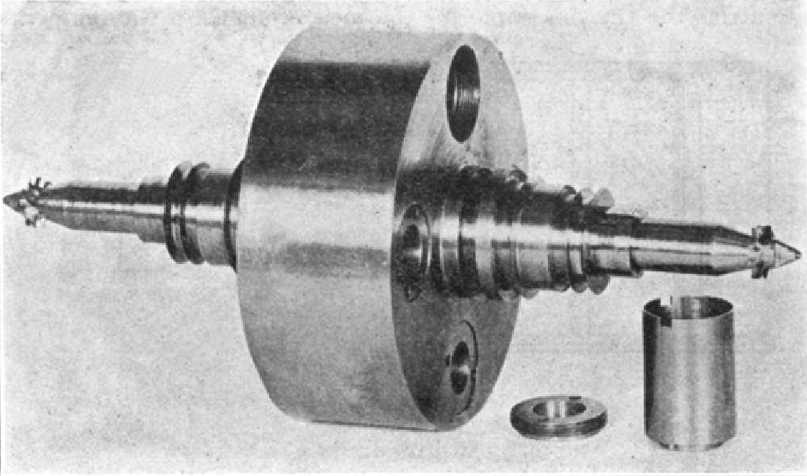
\includegraphics[height=0.3\linewidth,valign=t]{figures/ultracentrifugation_device.png} &
        b)                                                                                      &
        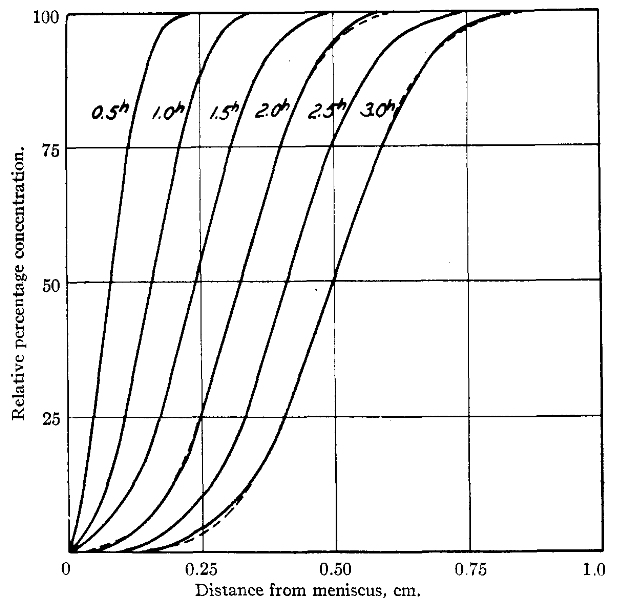
\includegraphics[height=0.3\linewidth,valign=t]{figures/ultracentrifugation_results.png}
    \end{tabular}

    \caption{a) Rotor from an ultracentrifuge. b) Haemoglobin concentration profiles from an early AUC experiments with rotor spinning at 42'000rpm or 104'000 G.
        Profiles derived from photographs taken at 30 minute intervals are compared with Lamm equation predictions (dashed).
        Reprinted with permission from \cite{Svedberg_1927}.
        Copyright 1927 American Chemical Society.
    }
    \label{fig:auc_diagram}
\end{figure}

Analytical Ultracentrifugation (AUC) is one of the oldest techniques in the domain of colloidal science receiving a Nobel prize in 1926.
In AUC a colloidal suspension is put inside a rapidly rotating centrifuge to increase the sedimentation rate of the molecules (current centrifuges spin with G-forces as large as 10'000G).
Inside the centrifuge rotor a small window allows for optical measurements of either absorption or transmission (in recent models involving multiple wavelengths) which change as a result of concentration variation.

Changes of concentration inside the container are governed by the Lamm equation containing the divergence of two currents
\begin{equation}
    \frac{\pd \phi}{\pd c} = \nabla \cdot \left( \underbrace{D \nabla \phi}_\text{diffusion} + \underbrace{s \omega^2 \mathbf{R} \phi}_\text{sedimentation} \right).
    \label{eqn:lamm-equation}
\end{equation}

Derivation of the $s$ and $D$ values from experimental, time-dependent concentration profiles is done via a fitting procedure which requires efficient solution schemes for the PDE~\eqref{eqn:lamm-equation}\cite{Demeler_2016,Cao_2005}.
Finite element method combined with nonlinear least-squares techniques and Monte-Carlo based error estimation allows gives both values and uncertainties of the $s$ and $D$ values which can be used to determine other molecular parameters such as $R_h$ or molecular mass.

\subsection{Fluorescence Correlation Spectroscopy}
\label{sec:FCS}

The overview of the Fluorescence Correlation Spectroscopy (FCS) technique follows that of \textcite{Tompson_2002} and \textcite{Gregor_2008}.
The FCS method, introduced about 50 years after invention of AUC, relies on temporal analysis of fluorescence signal to determine properties of the studied sample.
These include the hydrodynamic size (relevant to this work), but it is also possible to determine adsorption or reaction kinetics using this method.

In case of diffusion constant measurements a very dilute sample of studied molecule (typically marked with an added fluorophore) is illuminated by a laser inside a confocal microscope.
Excited fluorophore then emits light back through the microscope but at a slightly shorter wavelength (due to Stokes shift) which reaches the detector shielded from laser light with a dichroic mirror (cf \ref{fig:fcs_diagram}).

Recorded fluorescence signal $F(t)$ is time dependent since the number of molecules inside the laser beam changes in time due to diffusion.
FCS experiments perform best when at each moment expected number of excited molecules is close to one giving largest relative fluctuations of the fluorescence signal.

\begin{figure}[h]
    \centering
    \begin{tabular}{llll}
        a)                                                                     &
        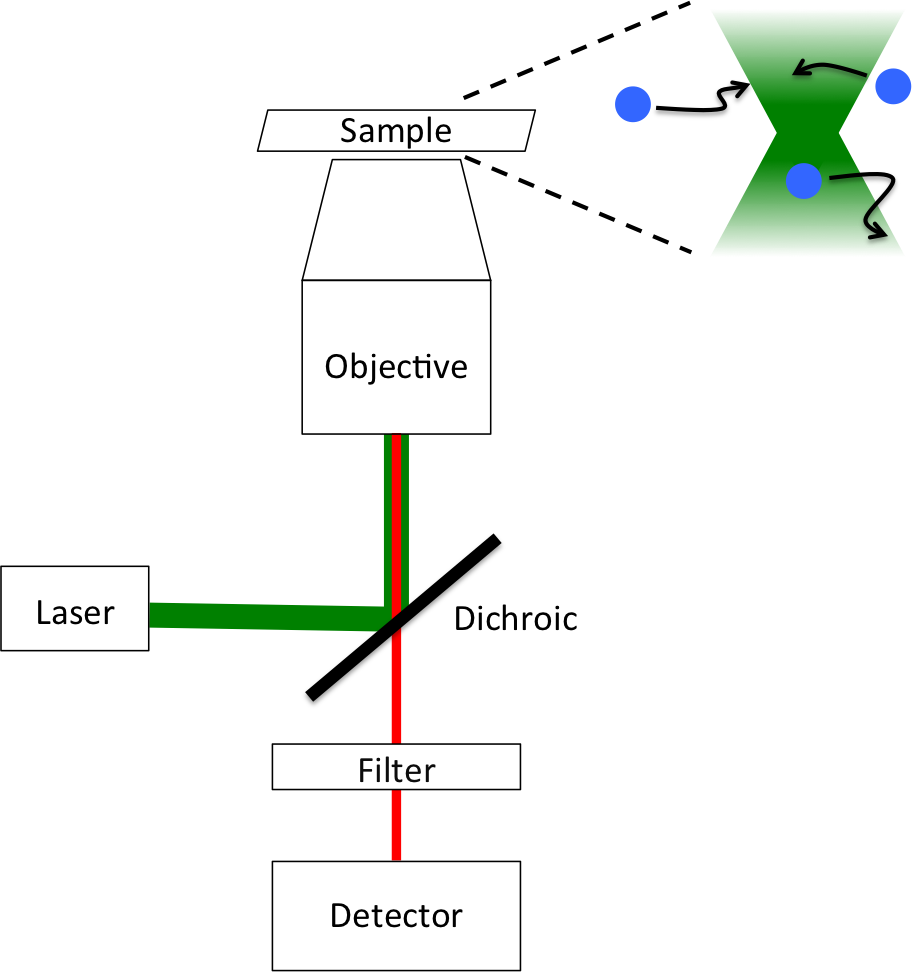
\includegraphics[height=0.3\linewidth,valign=t]{figures/fcs_setup.png} &
        b)                                                                     &
        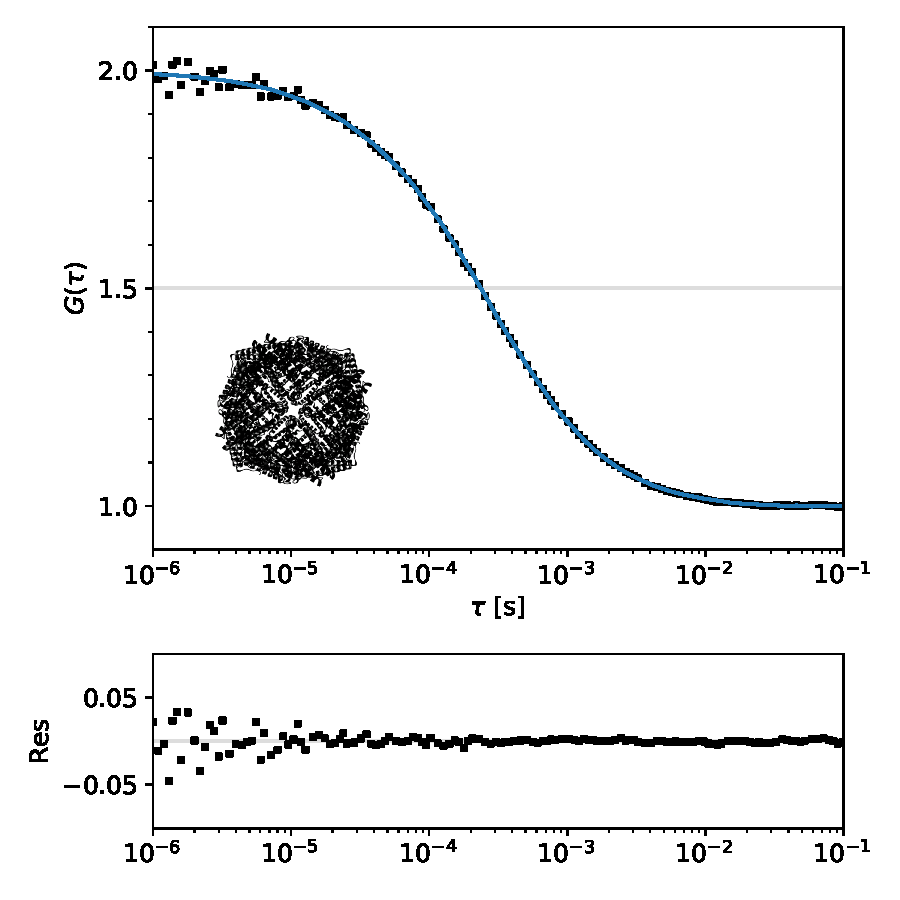
\includegraphics[height=0.32\linewidth,valign=t]{figures/fcs_data_and_fit.pdf}
    \end{tabular}

    \caption{a) A typical FCS setup diagram  b) Fluorescence correlation spectroscopy (FCS) data fit with a model for 3d diffusion.
        By Mllyjn CC BY-SA 3.0 TODO-REPLACE-WITH-AN-DATA-FROM-ARXIV} \label{fig:fcs_diagram}
\end{figure}

The frequency of the fluctuations due to diffusion can be quantified (and thus used to derive the diffusion coefficient) by considering signal autocorrelation function $G(\tau)$ given by 

\begin{equation}
    G(\tau) = \left< F(t) F(t-\tau) \right>
\end{equation}
with $\left< .
    % G(\tau) = \frac{\left< F(t) F(t-\tau)\right>}{\left< F(t)^2 \right>} - 1 %% Definition in Nancy Tompsons book
    \right>$ denoting time average.
This function is composed of two terms -- constant background (in case of non-interacting molecules) term due to photos coming from two different molecules and a delay dependent term quantifying probability of detecting a photon from the same molecule again.
For simplicity of this overview let's focus only on the last term.

Suppose for simplicity that a position-dependent probability of excitation describing the shape of the excitation volume can be described by a axisymmetric Gaussian profile $U(\mathbf{r})$ given by
\begin{equation}
    U(\mathbf{r}) = \kappa \exp\left( - \frac{2}{a^2} \left( x^2 + y^2 \right) - \frac{2}{b^2} z^2 \right) \label{eqn:excitation_profile}
\end{equation}
with $\mathbf{r} = [x,y,z]$ and $\kappa$ is some overall constant.

If we now consider the Green's function $g(\mathbf{\rho},\tau)$ of the diffusion problem given by 

\begin{equation}
    g(\mathbf{\rho},\tau) = \frac{1}{(4\pi D \tau)^{3/2}} \exp\left( - \frac{|\rho|^2}{4 D \tau}\right)
\end{equation}

we can express the autocorrelation function according to 

\begin{eqnarray}
    G(\tau) & = & \int \int U(\mathbf{r} + \mathbf{\rho}) g(\mathbf{\rho},\tau) U(\mathbf{r}) \dd \mathbf{r} \dd \rho \\
            & = & \frac{\pi^{3/2}}{8} \frac{a^2 b}{(1+4 D \tau / a^2)\sqrt{1+4D\tau/b^2}} \label{eqn:fcs_theory}
\end{eqnarray}

since the parameters $a$ and $b$ cannot be known a priori one typically fits a simplified expression 

\begin{equation}
    G(\tau) = G(0) \left( \left(1+\frac{\tau}{\tau_D}\right) \left(1 + \gamma \frac{\tau}{\tau_D}\right)^{1/2} \right)^{-1} + G(\infty) \label{eqn:fcs-autocorrelation}
\end{equation}
where $\gamma$ quantifies the aspect ratio of the excitation volume and $\tau_D$ characteristic time of the diffusion.
We can obtain diffusion coefficient $D$ from the residence time by comparing a reference sample of known $D$ and computing a ratio.

\subsection{Small Angle X-ray Scattering}
\label{sec:SAXS}

This section follows notation of \cite{Hermann_2008}.
Another experimental technique is based on the analysis of the X-ray scattering on the colloidal particles as a function of the beams deflection vector $\mathbf{q}$ defined as a difference between incoming wave vector $\mathbf{k}_i$ and scattered wave vector $\mathbf{k}_s$.

\begin{figure}[h]
    \centering
    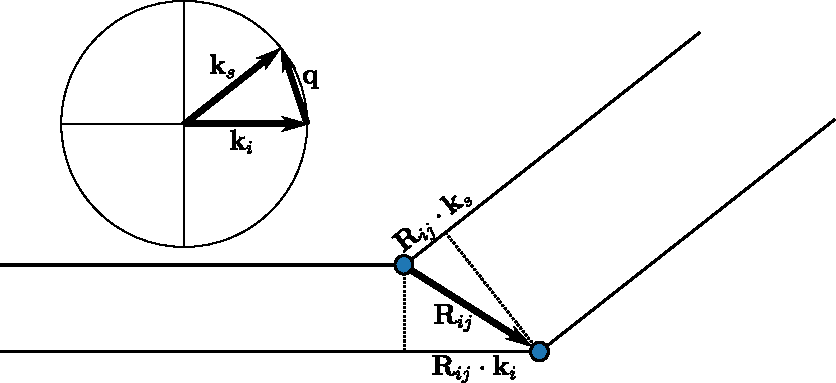
\includegraphics[width=0.6\linewidth]{figures/scattering_diagram.pdf}
    \caption{Phase shifts in Born approximation.}
    \label{fig:saxs_diagram}
\end{figure}

For colloidal particles the Born approximation of single-event scattering (as show in fig.~\ref{fig:saxs_diagram}) is a sufficient description to model experimental data.
Within this approximation the scattering pattern is computed as an interference pattern of the scattered signals from different scattering sites due to phase shift $\Delta \Phi$ resulting from difference in optical path length.

\begin{equation}
    \Delta \Phi = \mathbf{R}_{ij} \cdot (\mathbf{k}_s - \mathbf{k}_i) = \mathbf{R}_{ij} \cdot \mathbf{q}
    \label{eqn:scattering-phase-shift}
\end{equation}

We can express the complex amplitude of the scattered wave $A(\mathbf{q})$ as a Fourier transform of the scattering intensity distribution $\rho(\mathbf{r})$.

\begin{equation}
    A(q) = A_0 \int \rho(\mathbf{r}) \exp(i \mathbf{q} \cdot \mathbf{r}) \dd \mathbf{r} \label{eqn:scattering-amplitude-integral}
\end{equation}

Since the observed intensity on the screen $I$ is proportional to the squared absolute value of the wave amplitude $I(\mathbf{q}) \propto |A(\mathbf{q})|^2$ we can express $I(\mathbf{q})$ as a double integral 

\begin{eqnarray}
    |A(\mathbf{q})|^2 & = & A A^{*}                                                                                                                                        \\
                      & = & A_0^2 \int \int \rho^{*}(\mathbf{r}') \rho(\mathbf{r}'') \exp(i \mathbf{q} \cdot (\mathbf{r}'-\mathbf{r}'')) \dd \mathbf{r}' \dd \mathbf{r}''.
    \label{eqn:intensity-profile-integral}
\end{eqnarray}

If we assume that the scattering sites are point-like we can express the scattering density distribution as a sum of Dirac distributions $\delta$ centred at locations of scattering sites $\mathbf{s}_i$ 

\begin{equation}
    \rho(\mathbf{r}) = \sum_i \rho_i \delta(\mathbf{r}-\mathbf{s}_i)
\end{equation}
where $\rho_i$ gives scattering intensity on site $i$.
Changing the integral \eqref{eqn:intensity-profile-integral} to a double sum 

\begin{equation}
    I(\mathbf{Q}) = A_0^2 \sum_i \sum_j \rho_i \rho_j \exp(i \mathbf{q} \cdot (\mathbf{s}_i - \mathbf{s}_j))
\end{equation}

Inside the colloid the distribution of orientations of the macromolecules with respect to the lab frame is invariant under action of rotations.
For a vector $\mathbf{v} = \mathbf{s}_i - \mathbf{s}_j$ this simply implies $\mathbf{v}$ distributed uniformly on a sphere and its projection onto a vector $\mathbf{q}$ distributed uniformly on an interval according to orange slicing theorem\footnote{the orange slicing theorem: if you slice an orange into slices of equal thickness each slice has the same share of the orange peel} giving 

\begin{eqnarray}
    \left< I(\mathbf{Q}) \right> & = & A_0 \sum_i \sum_j \rho_i \rho_j \int \exp(i Q s) \mathbb{I}(|s| < |\mathbf{s}_i - \mathbf{s}_j|) \dd s \\
                                 & = & A_0 \sum_i \sum_j \rho_i \rho_j \operatorname{sinc}(|Q||\mathbf{s}_i - \mathbf{s}_j|)                  \\
                                 & = & A_0 \sum_i \sum_j \rho_i \rho_j \operatorname{sinc}(|Q||\mathbf{R}_{ij}|)
\end{eqnarray}

Thus the prediction of the scattering intensity of in a SAXS measurement of a colloidal suspension reduces to the computation of the distance matrix $R_{ij}$ between scattering sites given the values of scattering intensities $\rho_i(q)$.
In case of elastic macromolecules the scattering signal is simply averaged over an ensemble of possible molecular conformations.
With the help of tabulated values of scattering intensities of each amino-acid obtained by \textcite{Tong_2016} a python package \code{saxs_single_bead} was developed.

\chapter{Discussion}
\section{Experimental and theoretical challenges}
Much of theoretical enthusiasm in developing complex models, with a multitude of interactions is hampered by an insufficient quantity or quality of experimental calibration data, necessarily required for determination of molecular 'material constants'.
In the polymer science domains where data is plentiful (such as the area of globular proteins that can be readily measured by, for example, x-ray crystallography techniques), significant numerical progress could and was made using machine learning techniques leading to a celebrated example of AlphaFold \cite{Jumper_2021} reaching even pop-science recognisability.

Progress in the domain of elastic molecules is much more modest, even though they constitute a large proportion of proteins\cite{Ward_2004} and play an important role in multiple bio-relevant processes, such as the functioning of the COVID-19 virus\cite{Rozycki_2022} (to name just one example particularly resonant in 2023).
In the opinion of the author this progress is (at least in part) determined by the amount of readily available experimental data -- compare over 200 thousand conformations available in the Protein Data Bank\cite{rcsb_org} with not even 100 high quality measurements of the diffusion coefficients of the IDPs we were able to extract from published works\cite{Waszkiewicz_2024_mda} or 118 proteins in the Small Angle Scattering Database\cite{sasdb_org}, or 462 proteins in the Protein Ensemble Database\cite{proteinensemble_org}.

For the author the experimental challenges of studying bio-macromolecules have been an eye opening lesson in patience.
The excellent work on biosynthesis of the groups at Baylor College of medicine and Institute of Physics of Polish Academy of Science should not be underestimated.
These two collaborations give an overview of many experimental challenges: failure or success of initial biosynthesis, obtaining correct concentrations, through purification from by products of biosynthesis and the stability of the resultant molecular constructs to practical obstacles such as replacing discontinued lab equipment and cross border shipping.

Even if everything lines up and one obtains a good sample of the molecule to study the measurement itself is no easy task either.
Both AUC and FCS methods rely on time-series analysis of an optical signal - in that sense they are both indirect methods requiring model fitting within the experimental procedure as outlined in \ref{sec:AUC,sec:FCS}.
This complicates the analysis of the direct measurement error (uncertainty of a single measurement), with the current Monte-Carlo based AUC analysis method providing no uncertainty estimates for samples of high purity.
Single measurement error, however, is not the only and not even a leading source of uncertainty in the measurements of the diffusion (and sedimentation) properties of the molecules.
Since buffer conditions, concentration and even time from synthesis\cite{Nag_2011} affect the final outcome these have to be incorporated into error analysis to arrive at compound value of confidence interval of the measurements.
Some authors, unfortunately, do not provide any error estimates\cite{Poznar_2017,Khaymina_2007} and most of them do not discuss multiple sources of error.

Variety of bio-chemical insights into (both folded and disordered) protein behaviour invites phenomenological models to use many covariates in explaining hydrodynamic size of these molecules.
A specific example of one such insight could be the relative rigidity of polyhistidine fragments and tags, their presence (or more simply share of histidines in the totality of amino-acids forming a molecule) is sometimes used as a explanatory variable in a process of phenomenological modelling \cite{Tomasso_2016,Marsh_2010}.
As the data concerning hydrodynamic properties of IDPs is scarce and direct intervention in the protein sequence can be prohibitively expensive since synthesis of each new protein construct can take months we arrive at an issue more familiar to the social scientists than physicists - available information forms essentially an observation study where correlation is difficult to separate from causation \footnote{ This is in contrast to a typical physics experiment, akin to a randomised-controlled trial in social setting, where experimenter is free to chose value of control variable and measure the outcome.
    %
    In the example study of his-tag influence we can't simply, randomly separate proteins into two groups and add/remove his-tags as required.
}.
Even if we perform all of the statistical analyses correctly and we observe a statistically significant correlation between, for example, presence of a his-tag and increase in hydrodynamic size how can we be sure that it is not simply the case of a confounding cause?
One can easily imagine a scenario where compact proteins containing his-tag are simply harder to synthesise and thus we form our phenomenological conclusion based on a distorted sample (selection bias).
Correlations estimated this way can even have opposite sign to the real causal effect (which is what we're really trying to estimate)!
A comprehensive (and approachable) overview of causal vs correlational discrepancies in observational studies can be fond in \textcite{Cinelli_2022}.
Until and unless we arrive at a very large dataset of hydrodynamic properties of (a bias free, representative subset of) IDPs first principles theoretical models should take precedence over phenomenological models (not just because of their precision as we show in \textcite{Waszkiewicz_2024_mda}), but because they correctly model causal dependency between the covariates of interest and hydrodynamic size.
These models come in two flavours -- atomistic and coarse grained.

Atomistic methods of can sometimes be used\cite{Karplus_1990}, but they require either simulating the surrounding water molecules explicitly, which is very computationally intensive, or an implicit solvent scheme.
Both approaches pose significant numerical challenges \cite{Frenkel_2001}.
Even if simulations are in principle feasible, obtaining 10-100 millisecond long trajectories with this method which would enable the direct computation of the long-time diffusion coefficient are prohibitively expensive.

Coarse grained methods employ larger units (in case of proteins typically amino acid residues) as building blocks for the structure prediction scheme.
These are combined with a separate hydrodynamic model to predict diffusion coefficient.

\section{Approaches to Predicting Diffusion Coefficients in the Hot and Cold Limits}

As outlined, tackling the problem directly, even within a coarse-grained perspective, still presents numerical challenges.
Moreover, identifying a minimal model capable of reproducing experimentally observed variations in diffusion coefficients is inherently valuable.
This capability provides a direct interpretation of the observed variability through a restricted set of molecular mechanisms.

In the context of molecular dynamics, a convenient method for expressing dimensionless numbers is through lengthscale ratios, which quantify the respective ranges of different interactions within the molecule.

In our case, the lengthscales of interest include the persistence length $P = \frac{EI}{k_B T}$ (capturing elastic forces proportional to rigidity $EI$ in relation to Brownian forces proportional to fluctuation energy $k_B T$), the building block size (quantifying excluded volume interactions), and the Debye length (quantifying electrostatic interactions, scaling with the inverse square root of the ionic strength $C_s$ of the buffer).
Some values of these lengthscales, pertinent to the publications \cite{Waszkiewicz_2023_dna} and \cite{Waszkiewicz_2024_mda}, are outlined in Table~\ref{tab:lengthscales}.

\begin{table}[htbp]
    \centering
    \begin{tabular}{llrr}
        \toprule
        \textbf{Description} &
        \textbf{Scaling}     &
        \textbf{IDP [\AA]}   &
        \textbf{DNA [\AA]}                                              \\
        \midrule
        Length               & $L$                     & 2000 & 1000    \\
        Persistence length   & $P = EI / k_B T$        & 3    & 500     \\
        Building block       &                         & 4    & 3       \\
        Debye length         & $R_D \sim (C_s)^{-1/2}$ & 1    & 1       \\
        \midrule
        Applicable limit     &                         & hot  & cold(?) \\
        \bottomrule
    \end{tabular}
    \caption{Relevant length scales for the two studied problems.
        Length row represents typical values.
        Debye length computed for relevant (physiological) buffer conditions.
    } \label{tab:lengthscales}
\end{table}

First type of molecule investigated in this doctoral thesis are the DNA minicircles.
Here the need for assessing these values for each problem cannot be understated -- there is a factor $160$ difference in stiffness of protein linkers and DNA filaments.
Furthermore, the persistence length of DNA filaments is comparable to the length of the very short DNA minicircles under investigation by the group of Professor Lynn Zechiedrich at Baylor College of Medicine.
These minicircles were explored using two experimental techniques: CryoEM\cite{Irobalieva_2015} and analytical ultracentrifugation (AUC)\cite{Waszkiewicz_2023_dna}.

CryoEM images provide insight into the conformational properties of the DNA minicircles, while AUC measurements offer information on the hydrodynamic properties of the molecule.
To address our initial concern that the very large forces introduced by AUC methods (the molecules are sedimenting under $10\,000\mathrm{G}$) could affect the equilibrium shape properties of the DNA molecules, we conducted a study on the sedimentation of elastic filaments\cite{Waszkiewicz_2021_stability}.
The relative importance of elastic and buckling forces arising from sedimentation is quantified by the elasto-hydrodynamic lengthscale, $8\pi^3 \frac{EI}{L^2 g\rho}$, which for DNA is approximately $200\,000 $ \AA{} or $60$ kbp -- 200 times larger than the length of the minicircles of interest.
It is noteworthy that plasmids of that length are of biological interest, and additional care needs to be taken when studying them with AUC methods.

Moreover, the visual similarity between CryoEM figures from \textcite{Irobalieva_2015} and equilibrium configurations of twisted beams as described by \textcite{Coleman_2000} suggested that thermal fluctuations might have only a small influence on the overall behaviour of these molecules.
Consequently, we chose to model this problem in the 'cold' limit (cf.
Table~\ref{tab:tickmarks}), neglecting thermal fluctuations entirely and computing equilibrium configurations only (which is equivalent to working at negligible absolute temperature hence the name).
Subsequently, these configurations were treated as rigid bodies when determining the hydrodynamic radius, as detailed in \textcite{Waszkiewicz_2023_dna}.
The influence of thermal fluctuations was investigated further (after the publication) using the \code{pychastic} package, as outlined in Section \ref{sec:further_conclusions}.

\begin{table}[htbp]
    \centering
    \begin{tabular}{llll}
        \toprule
        \textbf{Manuscript}                                       &
        \textbf{Elasticity}                                       &
        \textbf{Thermodynamics}                                   &
        \textbf{Hydrodynamics}                                                                           \\
        \midrule
        DNA\cite{Waszkiewicz_2023_dna,Waszkiewicz_2021_stability} & \checkmark & .          & \checkmark \\
        IDP\cite{Waszkiewicz_2024_mda,Waszkiewicz_2024_trimer}    & .          & \checkmark & \checkmark \\
        Pychastic\cite{Waszkiewicz_2023_pychastic}                & \checkmark & \checkmark & \checkmark \\
        \bottomrule
    \end{tabular}
    \caption{Three domains of interest for the study of elastic molecules.
        Very high and very low stiffness of DNA and IDPs respectively allowed us to use simplified models.
    }
    \label{tab:tickmarks}
\end{table}

The second type of molecule investigated in this study were the intrinsically disordered proteins (IDPs).
These molecules exhibit much smaller stiffness, with an elastohydrodynamic length of approximately $2000$ \AA{} -- comparable to the molecule length.
This characteristic further justifies our initial concern regarding the potential influence of buckling forces arising in sedimentation on hydrodynamic sizes in some measurements.
Fortunately, the group led by prof.~Anna Niedzwiecka at the Institute of Physics, Polish Academy of Sciences, employs fluorescence correlation spectroscopy (FCS) instead of AUC, which does not introduce large force gradients on the molecule.

Similar to the DNA minicircle modelling, we compared lengthscales in the problem.
Given that the persistence length is comparable to the building block size, we decided to focus on the 'hot' limit of the problem, where elastic forces are disregarded relative to the thermal fluctuations (excluded volume interactions however do not vanish at high temperatures thus this approach can be treated as $\lim T \to \inf$ approximation, hence the name).
More precisely bending forces arising from the Ramachandran angles distributions were neglected, at the same time the forces that govern bond length were taken to be infinitely strong, this approach requires care when handling bond-angle distributions and some apparently paradoxical results can arise there as discussed in \textcite{Waszkiewicz_2024_trimer}.
We show that the intuitive distribution 'uniform on a sphere' indeed arises as a limit in the case of linear filaments (notably, a different distribution arises for molecules with loops as shown therein, with deviations in probability density that can be arbitrarily large).

Before estimating the diffusion coefficient of the IDPs, we aimed to assess the quality of the conformational ensembles resulting from our method, as described in more detail in \textcite{Waszkiewicz_2024_mda}.
For IDPs, one effective method for probing conformational properties without resorting to hydrodynamics is small-angle X-ray scattering (SAXS) described earlier in Section~\ref{sec:SAXS}.
We compared inter-domain distance data published in \textcite{Rozycki_2022} with data generated by the globule-linker model.
Additionally, we compared complete SAXS curves for ataxin-3 (PDB code \code{1yzb}) published in \cite{Lin_2017} with satisfactory results.
Further details regarding the \code{saxs_single_bead} package and the comparison are outlined in Section~\ref{sec:further_conclusions}.

\section{Combining Hot and Cold Approaches}
\label{sec:combining_hot_and_cold_approaches}
The two experimentally inspired problems, even though solvable to a satisfactory degree within the presented approximations, leave a desire to assess the size of the error introduced by these particular simplifications.
These error estimates can be compared either to the precision of the experimental data or to the estimates of other approximation errors in the model, such as approximations of the hydrodynamic mobility tensors.
This can guide the effort in further improvements to the numerical method; for example, should we first work on including thermal fluctuations to the conformations or rather improve hydrodynamic mobility tensor approximations?

When mobility tensors are simply modelled with the Rotne-Prager approximation (such as the tensors of the \code{pygrpy} package), the errors introduced there are of the order of 2\% (based on R8 test case of \cite{Zuk_2018}).

Assessing errors introduced by approximate conformer generation, whether in the hot ($T\to\infty$) or cold ($T\to0$) limit, necessitates simulating the ensemble at finite temperatures.
Various methods can be employed for this purpose, but a simulation grounded in physical principles holds particular appeal.
To achieve good performance, the Brownian Dynamics method was selected.
This approach relies on formulating the dynamical equation governing conformational changes in the form of a SDE.
Alternative formulations such as the Langevin equation or Fokker-Planck PDE are discussed in greater detail in \textcite{Waszkiewicz_2023_pychastic} and an introduction to subtleties of SDE is discussed in Section \ref{sec:SDE}.

Surprisingly, in 2022, the authors found that the only high-quality SDE integration package available was \code{differentialequations.jl} in Julia\cite{Rackauckas_2017}.
Since Julia is still not very popular among physicists (or at least not inside the soft-matter community) this resulted in frequent re-implementation of SDE integration methods for each problem and often re-implementation of the hydrodynamic interaction tensors as well (possibly due to the fact that the Rotne-Prager-Yamakawa tensors most frequently used in our group were originally implemented in Fortran\cite{Zuk_2018}).

We have tried to address this issue by making the packages \code{pychastic} (for SDE integration) and \code{pygrpy} (for Rotne-Prager-Yamakawa tensors) as easily accessible as we can -- single command installation, working on any reasonable linux distribution, MacOS and (as of 2023) even Windows10\cite{jax_on_windows}.
Additionally, we have invested substantial effort in creating straightforward yet realistic examples in the documentation.
This not only simplifies the learning curve but also aims to encourage wider adoption of our integration package.
For a comprehensive understanding of implementation and usage, please refer to the detailed information provided in \textcite{Waszkiewicz_2023_pychastic}.

The specific implementation of \code{pychastic} further streamlines the development of similar models by eliminating the need for explicit force specification.
Instead, users can now simply define the energy, and the forces can be derived programmatically using \code{jax.grad}.
This feature proved particularly advantageous in simulating shear-relaxed dynamics of DNA minicircles, where the energy depends on the non-local quantity of writhe ($Wr$), as discussed in detail in section~\ref{sec:further_conclusions}.

Answer to the correct development direction (in the opinion of the author) lies in future experimental data with resolutions capable of probing inaccuracies of the force-fields used or showing clear dependencies on buffer conditions such as temperature or ionic strength.
Such measurements are in the making and early results give a glimpse into the future DNA models\cite{Ranasinghe_2023}.

\section{Results not Included in Submitted Manuscripts}
\label{sec:further_conclusions}

\subsection{Thermal Effects on the Shapes of DNA Minicircles}

Utilising the \code{pychastic} package, we conducted simulations to explore the shapes of DNA minicircles at finite (room) temperatures and computed their apparent diffusion coefficient using the minimum dissipation method described in \textcite{Cichocki_2019}.

In these simulations, we assumed that torsional stresses in the DNA are relaxed.
Consequently, the total elastic energy $E_{el}$ of such a minicircle is given by
\begin{equation}
    E_{el} = \frac{1}{2} \int_0^L EI \kappa^2 + \left( \frac{2\pi (Lk - Wr)}{L} \right)^2 dl.
\end{equation}

Both $\kappa$ and $Wr$ can be computed from the shape of the centreline alone (or a suitable discretisation thereof), reducing the dimensionality of the problem compared to an approach where both the position and orientation of filament segments are simulated.
It is worth noting that simulating rotational dynamics, even of a single body, is a complex task, as outlined in \textcite{Waszkiewicz_2023_pychastic}.

Given that $Wr$ is a nonlocal quantity, the computation of forces from $E_{el}$ can be cumbersome.
Fortunately, this task can be accomplished with the assistance of \code{jax.grad}, which is compatible with the SDE solver \code{pychastic}.

This gives further insight into the intermediate region ($1 < Lk < 2.5$) where minicircles have multiple stable configurations at absolute zero temperature discussed in \textcite{Waszkiewicz_2023_dna}.

\begin{figure}[htbp]
    \centering
    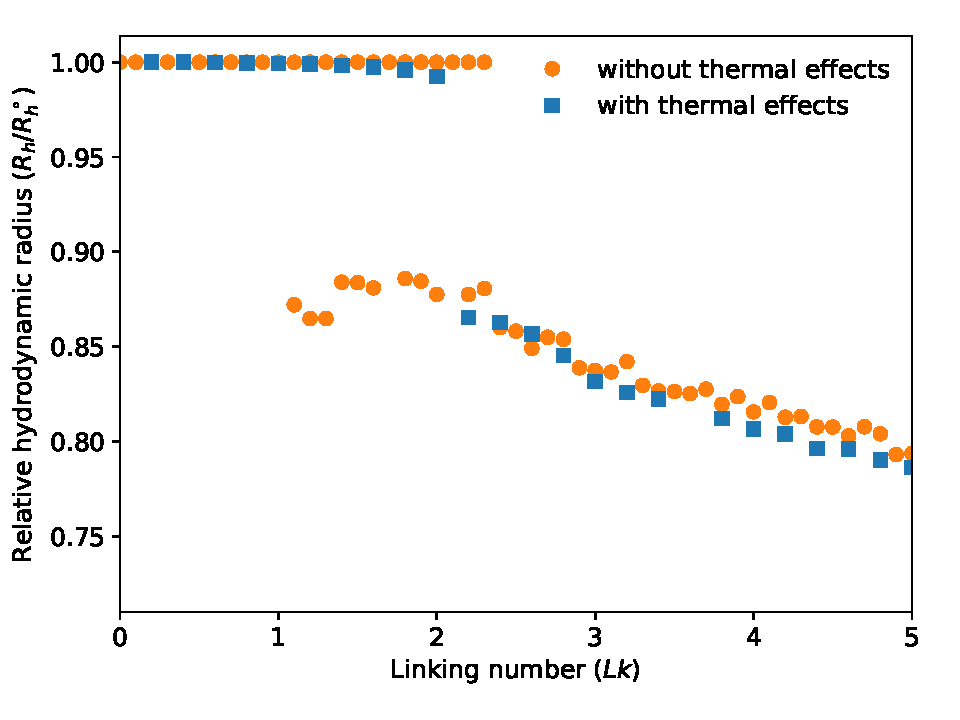
\includegraphics[height=0.5\linewidth]{figures/with_thermal_effects.pdf}
    \caption{Relative hydrodynamic radius of the 336bp minicircle as a function of the linking number.}
    \label{fig:thermalized_loops}
\end{figure}

It turns out that the effects of thermal fluctuations on the overall hydrodynamic radius outside of the intermediate region are negligible.
Moreover, the range of $Lk$ values for which the equilibrium ensemble contains both open configurations and configurations with self-contact is very small—less than 0.2 turns.
When considering the difference in total elastic energy between the flat circular configuration and the configuration with self-contact, one arrives at $\frac{\partial \Delta E}{\partial Lk} \approx Lk \frac{4\pi^2 \cdot 2}{3} \frac{P}{L} k_B T \approx 26 k_B T$, providing an estimate of the transitional region width of approximately $0.03$.
%TODO: redo this calculation and check
This contrasts starkly with CryoEM data\cite{Irobalieva_2015}, where a multitude of conformations were observed for a wide range of $Lk$ values.
One possible explanation for this discrepancy lies in the temperature dependence of the geometric properties of DNA, as hinted at by the results of \textcite{Ranasinghe_2023}.

\subsection{Comparing Conformations to SAXS Data}
The author would like to thank dr.
Bartosz Różycki for his guidance regarding experimental SAXS data.

As detailed in \textcite{Waszkiewicz_2024_mda}, computing the diffusion coefficient for a given IDP requires generating samples from the equilibrium ensemble.
To assess the quality of the conformer generation method independently of hydrodynamic modelling, we utilised available SAXS data.
One example of such a comparison is illustrated in Figure~\ref{fig:saxs_compare}, where experimental data from \textcite{Sicorello_2021} is compared with our implementation of the globule-linker model (\code{sarw-spheres}) combined with our implementation of the one-site-per-amino-acid scattering model (\code{saxs-single-bead}).
This model is based on form factors computed by \textcite{Tong_2016}.

\begin{figure}[htbp]
    \centering
    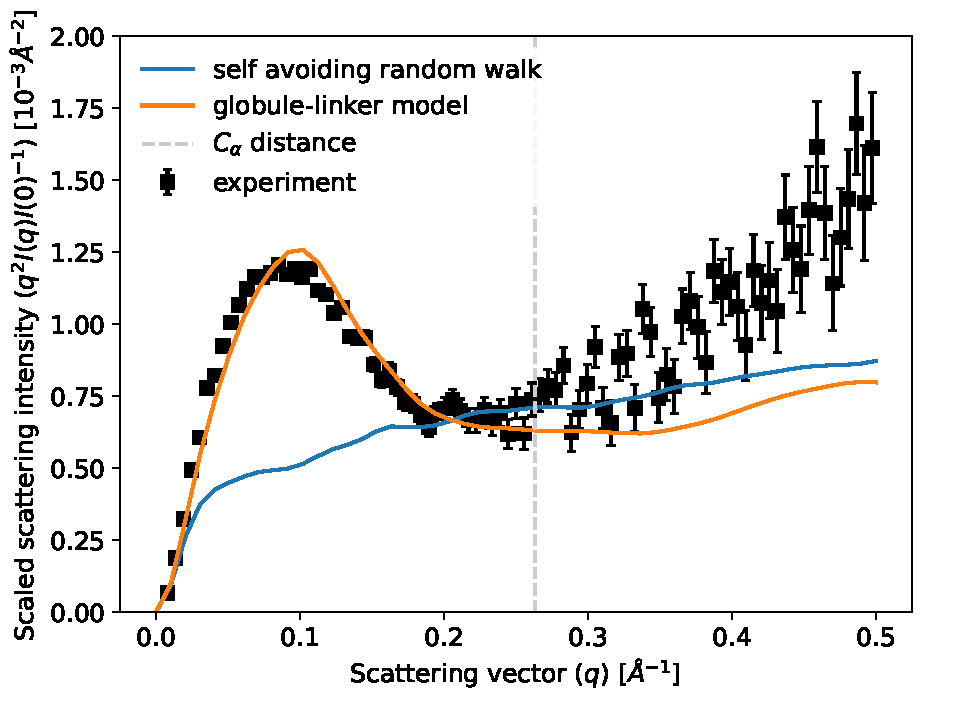
\includegraphics[height=0.5\linewidth]{figures/saxs_single_bead.pdf}
    \caption{Kratky plot generated using \code{saxs_single_bead} package for {ataxin-3} (pdb id \code{1yzb}) compared with experimental data from \textcite{Sicorello_2021}.}
    \label{fig:saxs_compare}
\end{figure}

The conformations used to predict the SAXS curve in Figure~\ref{fig:saxs_compare} were generated using the globule-linker engine, with the globule replaced by crystallographically obtained data retrieved from the Protein Data Bank (PDB)\cite{rcsb_org}.
The excellent agreement in the range of scattering vectors corresponding to features larger than the $C_{\alpha}$ distance (small values of $q$) is a result of the combination of adequate modelling of both the rigid and flexible parts.

\section{Software packages}

\begin{table}[htbp]
    \centering
    \begin{tabular}{llll}
        \toprule
        \textbf{Package}        &
        \textbf{Description}    &
        \textbf{GitHub}         &
        \textbf{Docs}                                                                                                           \\
        \midrule
        \code{pychastic}        & SDE solver                          & \cite{gh_pychastic}        & \cite{rd_pychastic}        \\
        \code{pygrpy}           & Rotne-Prager mobility tensors       & \cite{gh_pygrpy}           & \cite{rd_pygrpy}           \\
        \code{sarw-spheres}     & Globule-linker conformer generator  & \cite{gh_sarw_spheres}     &                            \\
        \code{saxs-single-bead} & One site per amino-acid SAXS engine & \cite{gh_saxs_single_bead} & \cite{rd_saxs_single_bead} \\
        \code{pywrithe}         & Computing writhe of a curve         & \cite{gh_pywrithe}         & \cite{rd_pywrithe}         \\
        \bottomrule
    \end{tabular}
    \caption{Software packages developed in the course of preparation of this doctoral thesis.}
    \label{tab:packages}
\end{table}

\chapter{Main results of the thesis}
\clearpage

\begin{publicationpage}{Waszkiewicz_2021_hydrodynamic}{Hydrodynamic effects in the capture of rod-like molecules by a nanopore}
    \commentary{               
        Translocation of biomolecules through nanopores lies at the heart of many biological processes, such as cell signalling.
        It is a significant element of modern nanotechnology and sequencing techniques which give access to the structure of DNA or RNA in small quantities.
        Thus, it enables low-cost genotyping and testing without the need to resort to PCR amplification or chemical labelling.

        In a relevant experimental setup for DNA analysis, the efficiency of sequencing hinges on two critical factors: the translation speed through the nanopore and the capture radius of the nanopore.
        The complex process of translocation is now understood in great detail and has been studied extensively to assess the importance of multiple contributing factors.
        However, the process of approach and capture by a nanopore still poses a challenge.
        Existing models of capture mostly overlook hydrodynamic interactions which might play an important role when the DNA fragment is sufficiently close to the nanopore.
        This work aimed to fill this gap by discerning and examining the time scales associated with different modes of motion -- rotational and translational -- induced by different types of forces present in the system: Brownian fluctuations, electrostatic attraction to the pore, and hindering effects of hydrodynamic interaction with the wall.
        By the analysis of different regimes, we successfully identified the pore distance at which wall interaction terms exert a dominant influence and therefore should be accounted for in quantitative models.

        To perform the analysis, we constructed a simple coarse-grained model of an anisotropic, rod-shaped particle, representing the elongated nature of a DNA filament of length short compared to its persistence length.
        In such a case the molecules can be treated as a stiff rigid body, for which an approximate form of the mobility tensor in the presence of a wall has been proposed \cite{Lisicki_2016}.
        In this work, we performed scaling analysis to identify the regimes where different types of forces are dominant.
        We then calculated the trajectories of a model nanorod near a wall in Mathematica, incorporating the near-wall corrected mobility tensor, which takes into account both the anisotropy of the particle itself, and its coupling to the wall.
        In this study, the PhD candidate: co-developed the scaling analysis and the theoretical description, implemented the near-wall corrections to the mobility tensors and generated all numerical results and visualisations presented, participated in the analysis of results, prepared all figures, wrote the first draft and edited all subsequent versions.
    }

\end{publicationpage}
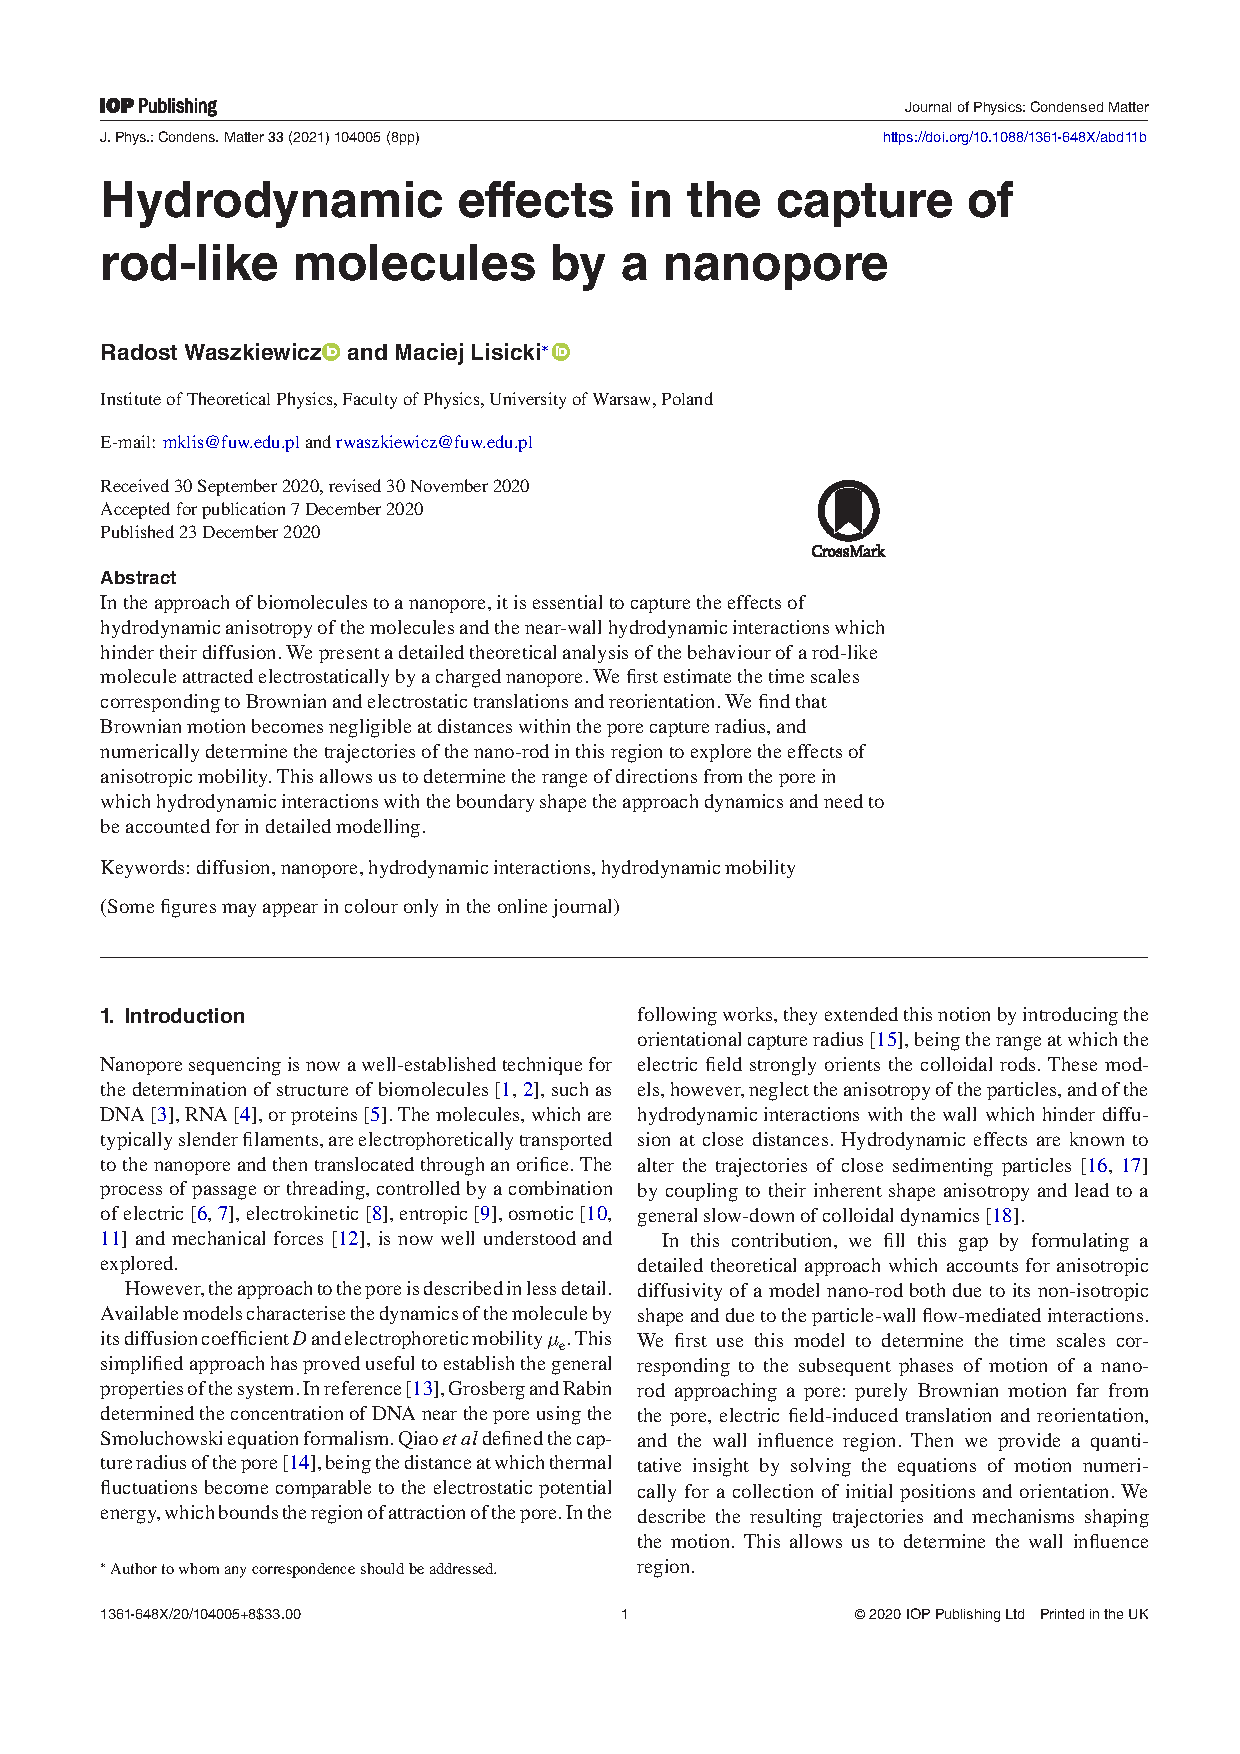
\includepdf[pages={-}]{publications/waszkiewicz_2021_hydrodynamic}

\begin{publicationpage}{Waszkiewicz_2021_stability}{Stability of sedimenting flexible loops}
    \commentary{
        Analytical Ultracentrifugation, a method for determination of hydrodynamic radius and effective density of a molecule, involves applying extremely high centrifugal forces to a colloidal suspension.
        This well established technique has been successfully used to measure various colloidal particles, however, its application to flexible macromolecules raises concerns over the influence of large forces (or more precisely large force gradients) imposed on the molecule.
        In extreme cases high values of compression in the fore of the sedimenting particle can lead to buckling in sedimentation processes.
        To address this concern, we focused on an idealised problem involving the sedimentation of a circular fibre, aiming to eliminate end-corrections from the buckling consideration.

        To determine cases where the buckling may occur we performed linear stability analysis within the Resistive Force Theory approximation, where the tension inside the loop at each moment can be simply described by a ordinary differential equation. 
        We calculated the evolution of the conformation of a sedimenting loop using a custom numerical integrator based on a truncated Fourier series.

        In this study, the PhD candidate: conducted a stability analysis of the PDE and computed the stability criterion using the proposed matrix method, generated all numerical results and visualisations presented, prepared all figures, wrote the first draft and edited all subsequent versions. Additionally they are a corresponding author.
    }
\end{publicationpage}
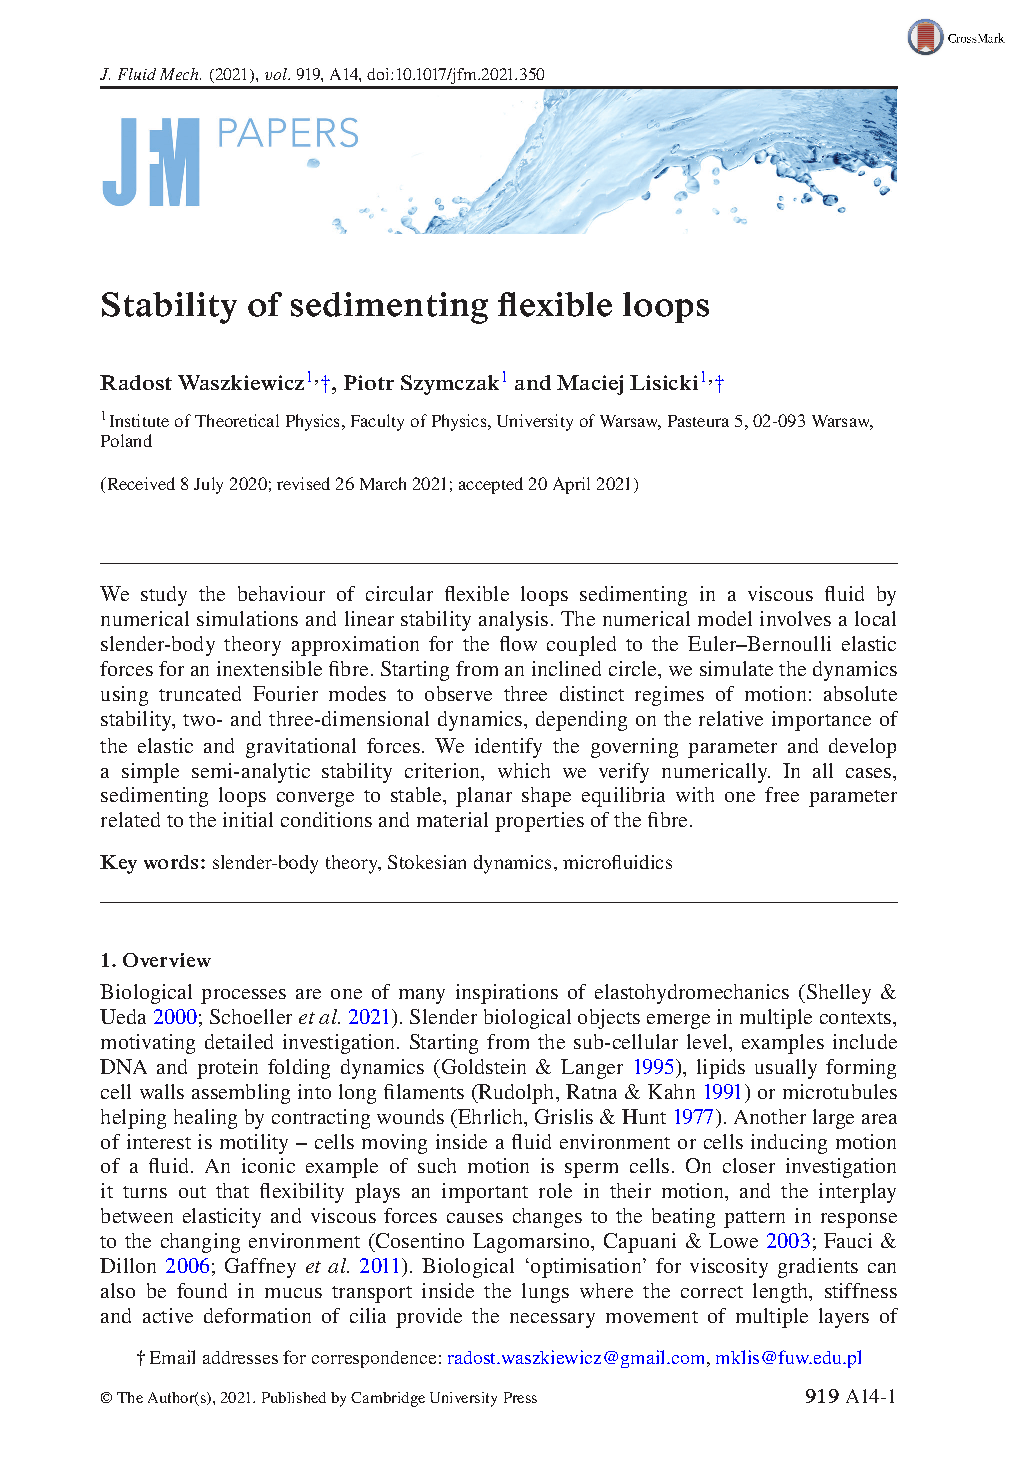
\includepdf[pages={-}]{publications/waszkiewicz_2021_stability}

\begin{publicationpage}{Waszkiewicz_2023_dna}{DNA supercoiling-induced shapes alter minicircle hydrodynamic properties}
    \commentary{
        Bio-relevance of the DNA requires little introduction. 
        Even though the basic structure of the DNA is well understood at least since the 1950s, undestanding the secondary structure of the DNA filament remains an imporant, but challegning task.
        Since the overall 3D conformation of the DNA can influence gene expression understanding the forces governing its elasticity is key.
        By using a selection of small DNA loops which differ only in the linking number we were able to measure conformational changes of the DNA via its hydrodynamic properties in the diffusive measurements.

        This study emerged from the collaborative efforts of three distinct groups.
        The first group, specialising in theoretical modelling, comprised the PhD candidate, Maria L Ekiel-Jeżewska, Maciej Lisicki, and Piotr Szymczak from the Warsaw University Physics Department and the Institute of Fundamental Technological Research, Polish Academy of Sciences.
        The second group, responsible for the biosynthesis of DNA minicircles, included Jonathan M Fogg, Daniel J Catanese Jr, and Lynn Zechiedrich from the Department of Pharmacology and Chemical Biology at Baylor College of Medicine.
        The third group, overseeing AUC measurements, was included Maduni Ranasinghe and Borries Demeler from the Department of Chemistry and Biochemistry at the University of Lethbridge.

        The choice of topoisomers of DNA minicircles as the subject of collaboration proved strategic.
        For the modelling group, the shared hydration properties among different topoisomers and their loop structure, as opposed to rods, facilitated a more straightforward modelling process.
        The biosynthesis group leveraged their prior experience in preparing these molecules, coupled with an interest in understanding the physical origins of changes in the bio-activity of writhed DNA.
        Lastly, for the AUC group, the remarkable sample stability of DNA minicircles allowed for numerous re-runs of experiments.

        In this study, the PhD candidate: proposed and implemented a numerical method to obtain equilibrium configurations of the supercoiled DNA minicircles. They computed the hydrodynamic properties of these configurations using GRPY, pygrpy, and Zeno software (with only Zeno being included in the published manuscript); wrote the first draft and edited all subsequent versions of the manuscript, produced all graphs and visualisations incorporated in the manuscript.
    }
\end{publicationpage}
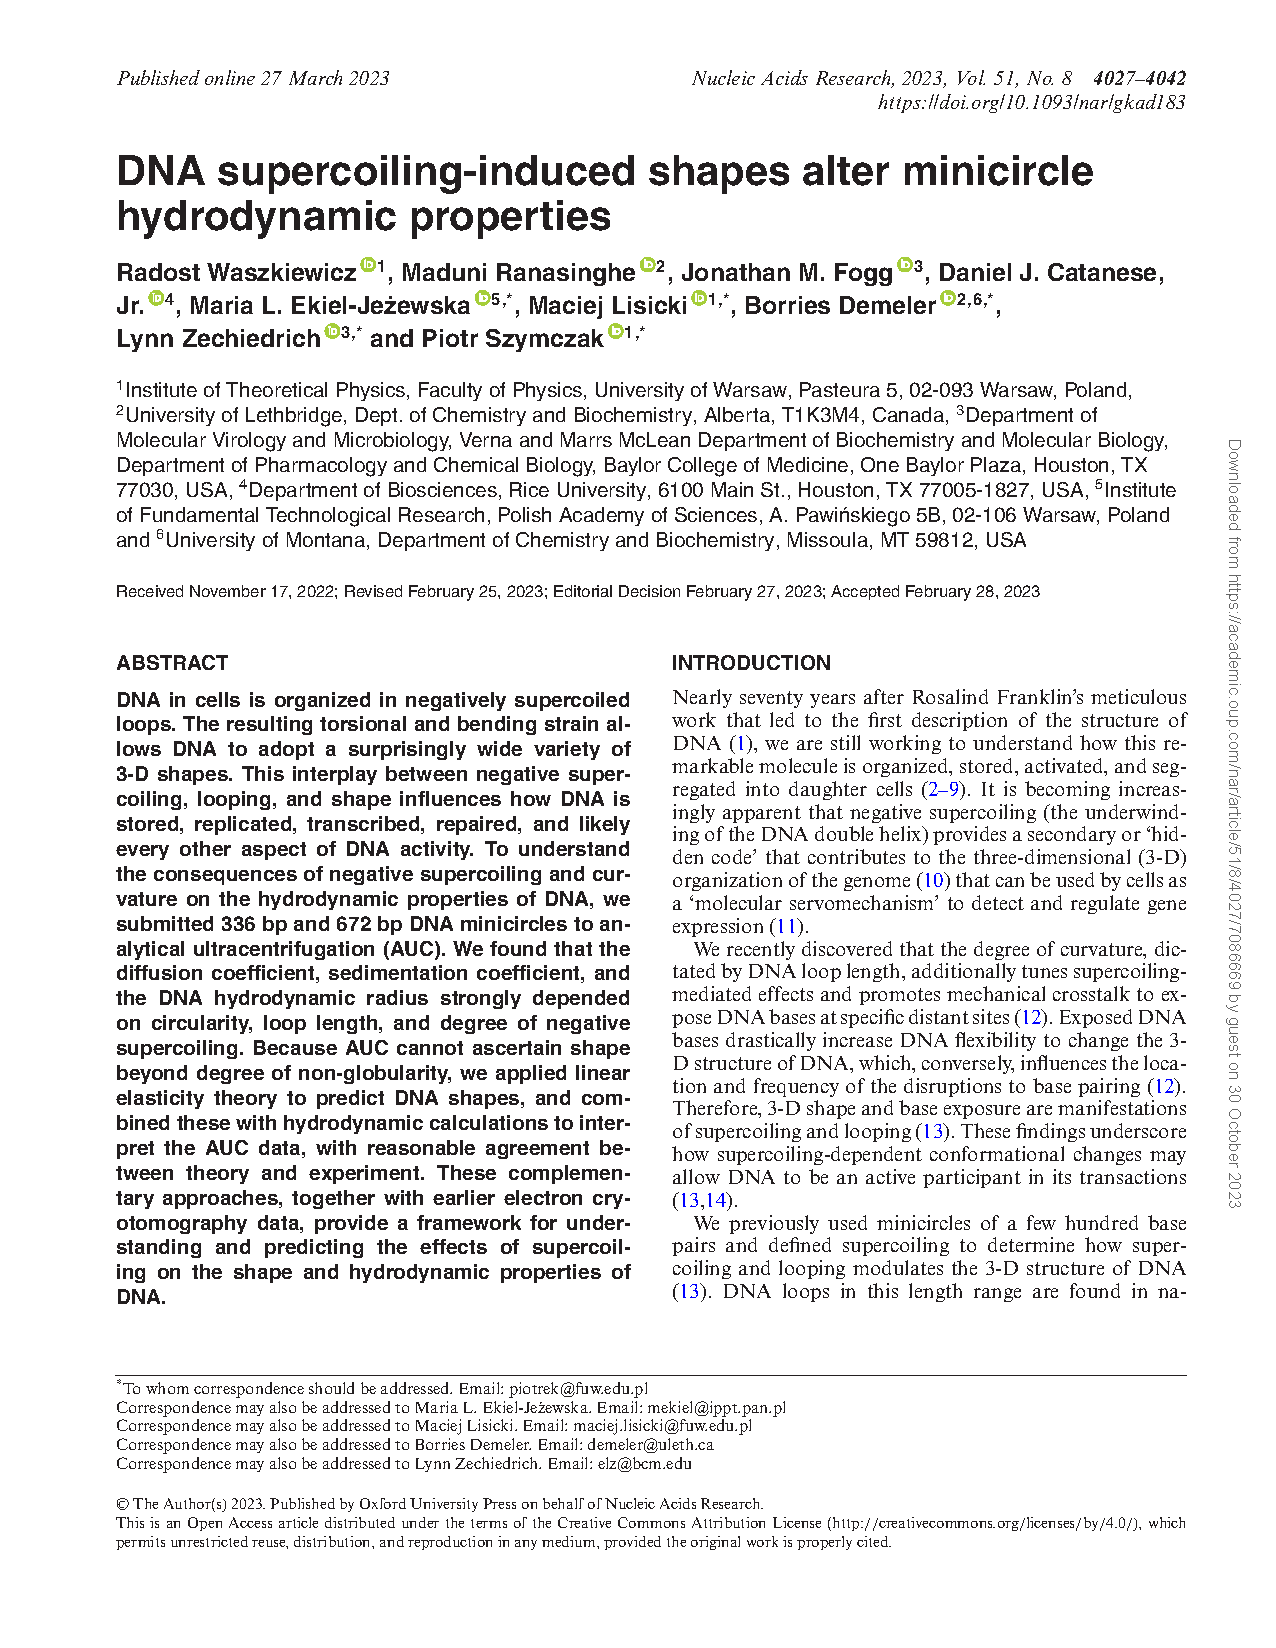
\includepdf[pages={-}]{publications/waszkiewicz_2023_dna}

\begin{publicationpage}{Waszkiewicz_2023_pychastic}{Pychastic: Precise Brownian dynamics using Taylor-Ito integrators in Python}
    \commentary{
        The major theoretical limitation in earlier studies revolved around the incomplete treatment of Brownian motion.
        In the case of \cite{Waszkiewicz_2021_hydrodynamic}, dynamics had to be simplified to a 2D case due to Mathematica's inability to handle full $SO(3)$ dynamics, as outlined in the publication below.
        Similarly, in \cite{Waszkiewicz_2023_dna}, the challenges arose from the nature of the Writhe quantity, leading to a non-local force field that made assessing the effects of thermal fluctuations on the shape of minicircles challenging.

        Addressing the treatment of Brownian motion through stochastic differential equations presented a well-posed mathematical problem.
        However, surprisingly, there was no readily available, easy-to-use solution, such as the package described in the publication below.

        In this study the PhD candidate: lead a small programming team, which included the author, Maciej Bartczak, and Kamil Kolasa, co-developed a Python package complete with documentation, examples, and tests, created test cases and debugging tools that facilitated the correction of multiple typos found in existing literature (outlined in the publication).
        Together with Maciej Lisicki, designed illustrative examples showcasing concrete applications of the tools developed during the thesis preparation.
        Additionally wrote the first draft and edited all subsequent versions of the manuscript.
    }
\end{publicationpage}
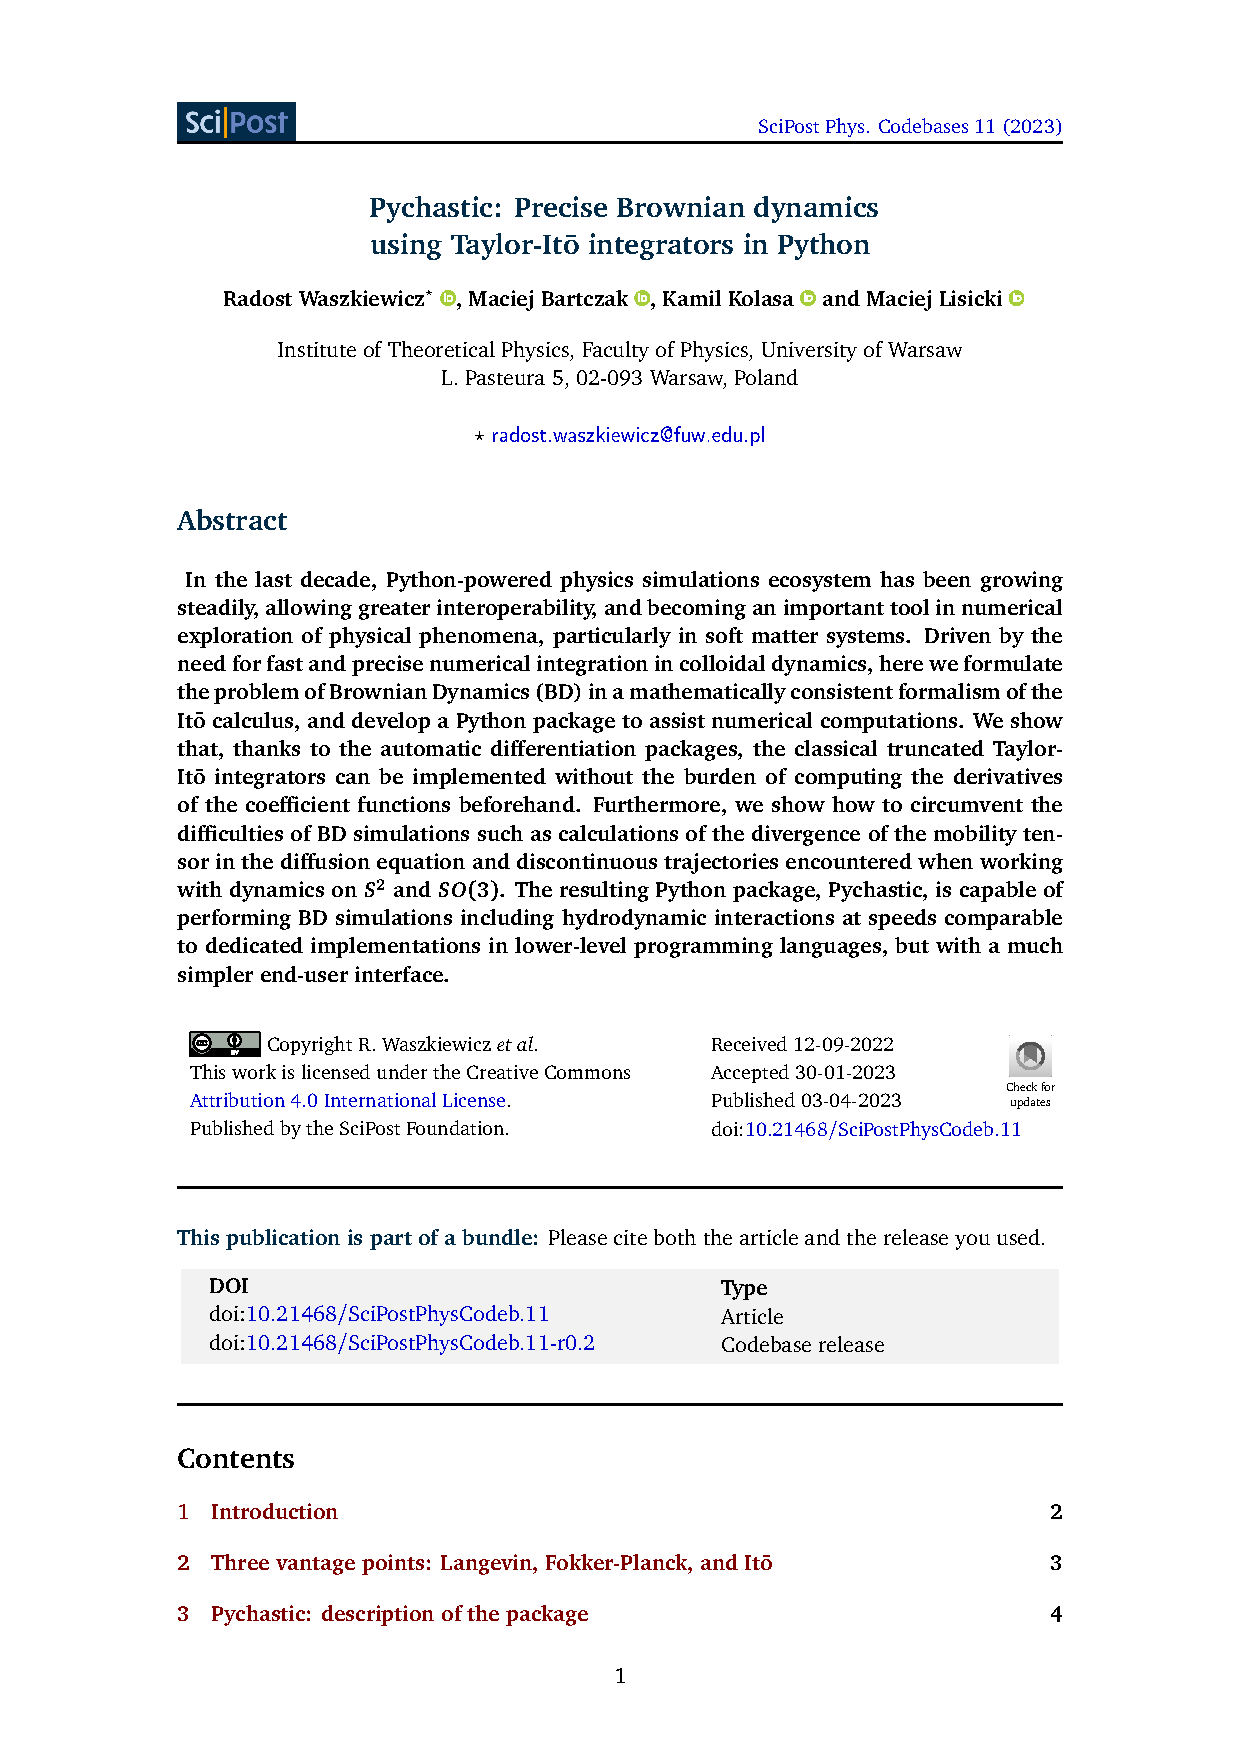
\includepdf[pages={-}]{publications/waszkiewicz_2023_pychastic}

\begin{publicationpage}{Waszkiewicz_2024_mda}{Minimum dissipation approximation: A fast algorithm for the prediction of diffusive properties of intrinsically disordered proteins}
    \commentary{
        Intrinsically Disordered Proteins (IDPs) constitute a large class of bio-relevant elastic macromolecules. TODO

        From a modelling perspective, intrinsically disordered proteins differ significantly from DNA.
        They consist of globular fragments connected with linkers, where the former are essentially rigid, and the latter are almost ideally flexible.
        Such proteins are ideal subjects for the application of the minimum dissipation approximation, specifically designed for the fast computation of diffusion coefficients for molecules exhibiting substantial conformational variability and parts of varying sizes.

        This study emerged from the collaborative efforts of two distinct groups.
        The first group, specialising in theoretical modelling, included PhD candidate, Bogdan Cichocki, Maciej Lisicki and Piotr Szymczak from the Warsaw University Physics Department.

        The second group, responsible for synthesis and FCS measurements, comprised Agnieszka Michaś, Michał K.~Białobrzewski, Barbara P.~Klepka, Maja K.~Cieplak-Rotowska, Zuzanna Staszałek, and Anna Niedźwiecka from the Institute of Physics of the Polish Academy of Sciences.

        In this study the PhD candidate: investigated the Flexible Meccano conformer generation scheme, implemented the python port \code{pygrpy} of the generalised Rotne-Prager mobility tensors (originally implemented in Fortran\cite{Zuk_2018}), implemented the globule-linker conformer generation scheme, performed the numerical calculations and statistical analysis to assess deviations between theory and experiment.
        Additionally wrote the first draft and edited all subsequent versions of the manuscript.
    }
\end{publicationpage}
\includepdf[pages={-}]{publications/Waszkiewicz_2024_mda}

\begin{publicationpage}{Waszkiewicz_2023_trimer}{TODO: toc title}
    \commentary{
        TODO - are we even including this?
        Performing theoretical calculations regarding equilibrium distributions of molecules with arbitrarily stiff bonds and numerical calculations using \code{pychastic} package to give illustrative examples of the discussed phenomena.
    }
\end{publicationpage}
%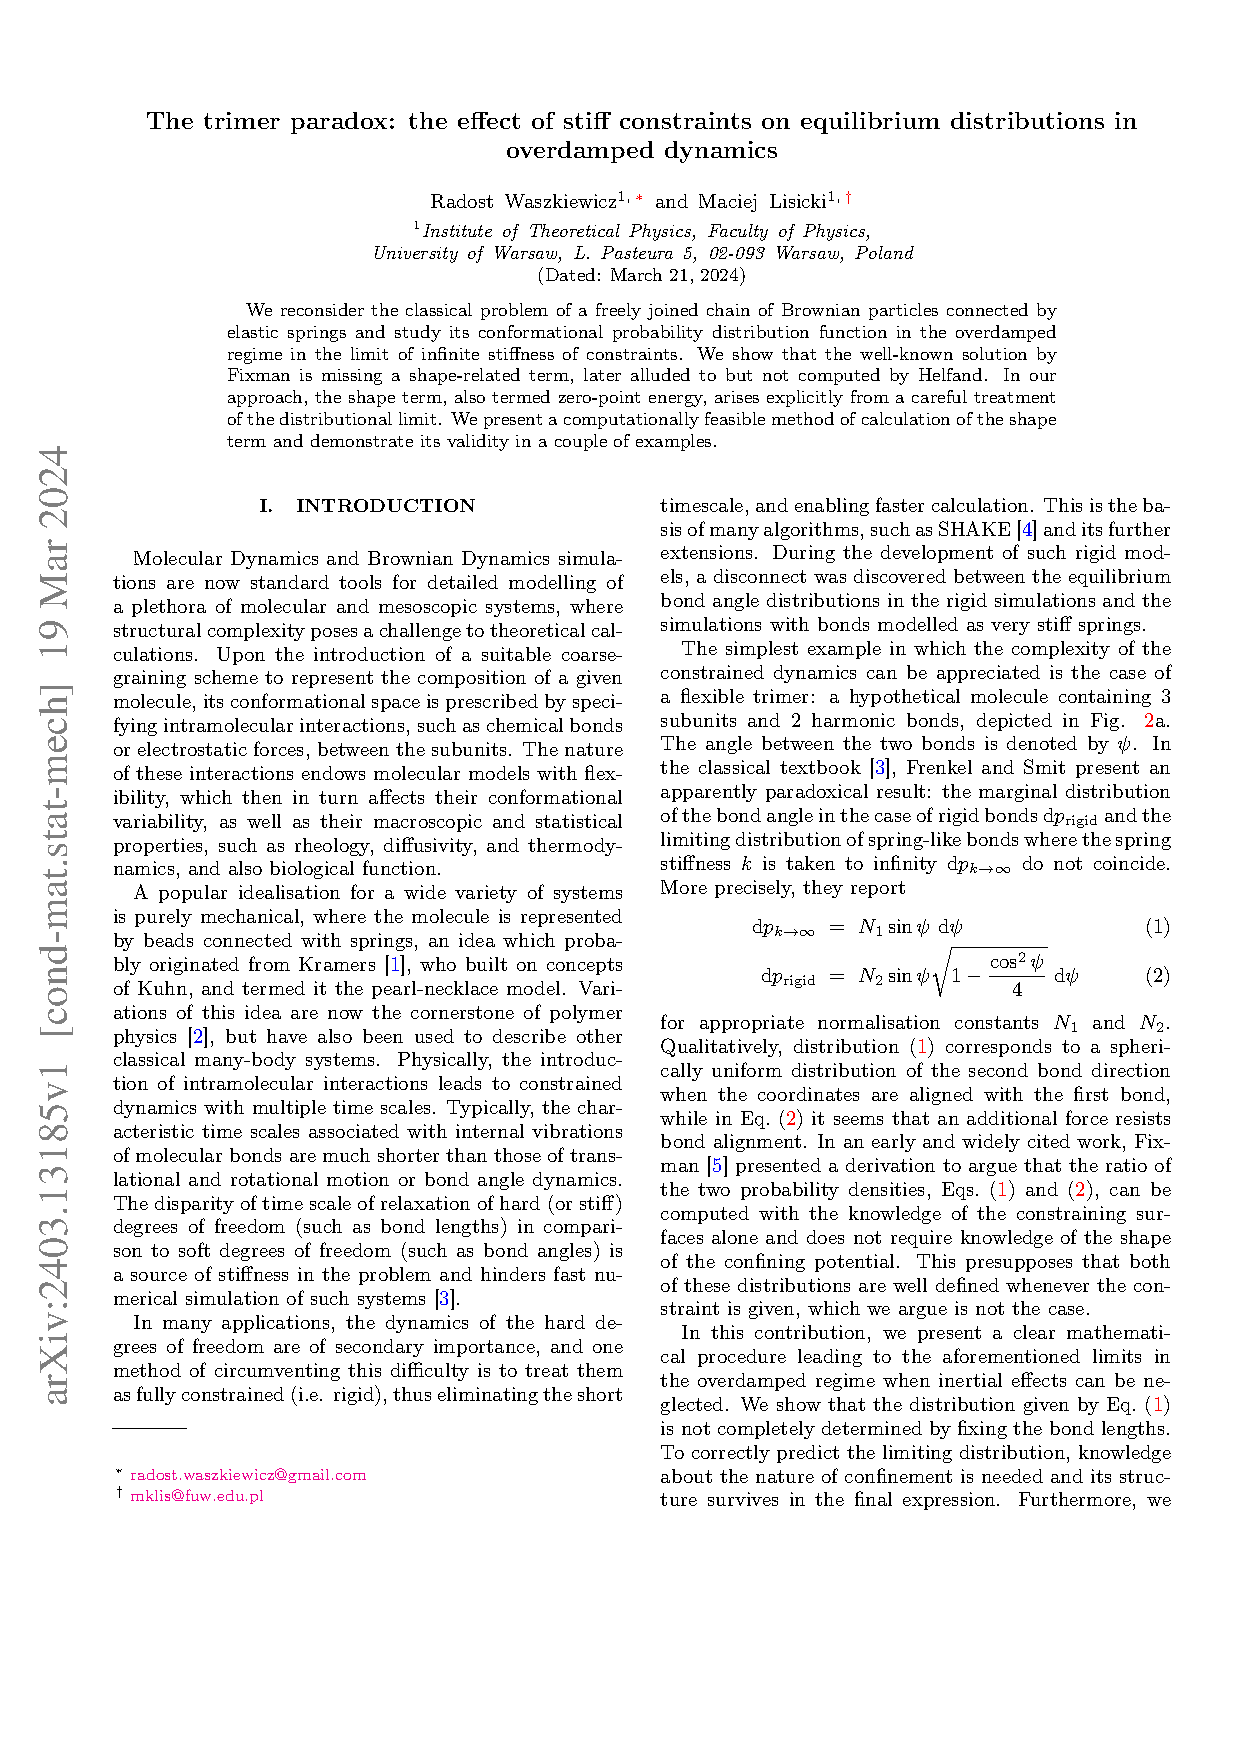
\includepdf[pages={-}]{publications/waszkiewicz_2024_trimer}

\chapter{Conclusions}

The objectives of the present thesis were twofold -- find theoretical approaches capable of modelling experimentally relevant macromolecules and provide a step towards a single, modular system capable of accommodating different coarse graining approximations and experimental techniques.

The results of this thesis show that such unified approach is possible and that it predicts diffusion coefficients of macromolecules with good precision.
The main achievements of this thesis can be summarised as follows:
\begin{enumerate}
    \item We have successfully predicted hydrodynamic radii of DNA loops at different values of linking number.
    \item We have successfully predicted hydrodynamic radii of many intrinsically disordered proteins from the largest to-date benchmark set.
    \item We have provided easy to use, well documented and publicly available Python implementations to all theoretically proposed methods (without compromising the prediction speed).
\end{enumerate}

Thus the presented method can be used as a numerically feasible null-hypothesis model in future investigations by multiple experimental groups with large deviations from its predictions being an indicator of new and exciting physical phenomena.
Additionally we hope that the theoretical soft matter physics community will be able to use the software prepared as part of the presented thesis in multiple ways.
Either in its current form for predicting diffusion coefficients of similar molecules or by taking advantage of its modular design by either extending its current capabilities or using its parts in isolation.

\printbibliography[heading=bibchapter]

\end{document}
